\documentclass[12pt,a4paper]{article}

\usepackage{iftex}
\ifPDFTeX
    \usepackage[utf8]{inputenc}
    \usepackage[T5]{fontenc}
    \usepackage[vietnamese]{babel}
    \usepackage{lmodern}
\else
    \usepackage{fontspec}
    \setmainfont{Times New Roman}
\fi
\usepackage{geometry}
\usepackage{longtable}
\usepackage{booktabs}
\usepackage{array}
\usepackage{enumitem}
\usepackage{hyperref}
\usepackage[table]{xcolor}
\usepackage{amsmath}
\usepackage{amssymb}
\usepackage{graphicx}
\usepackage{float}

\geometry{margin=2.5cm}
\hypersetup{
    colorlinks=true,
    linkcolor=blue,
    urlcolor=blue,
    citecolor=blue
}

% ── Trình bày bảng rõ ràng: tô màu xen kẽ từng dòng + giãn chiều cao dòng ──
\definecolor{rowalt}{gray}{0.90}
\renewcommand{\arraystretch}{1.3}

\begin{document}

% Bật tô màu xen kẽ cho mọi bảng (dòng tiêu đề trắng, thân bảng xen kẽ xám nhạt)
\rowcolors{2}{white}{rowalt}

\begin{center}
    \large\textbf{ĐỀ XUẤT DỰ ÁN HỆ THỐNG CƠ SỞ DỮ LIỆU PHÂN TÁN} \\[6pt]
    \Large\textbf{DISTRIBUTED DATABASE PROJECT PROPOSAL} \\[10pt]
    \small\textit{Mẫu đề xuất Dự án môn học Cơ sở dữ liệu phân tán (Distributed Database Project Proposal)}
\end{center}

\vspace{1cm}

\noindent\textbf{Hạn nộp (Due Date):} Tuần 3 (Week 3) --- 15/06/2026 \\
\noindent\textbf{Mã đề tài \& Phân loại (Project ID \& Category):} Topic \#112: Distributed Watermark Tracker (``Log Delay Compensator'') --- Category 3

\vspace{0.8cm}

% ─────────────────────────────────────────────────────────────────────────────
\section{Project Identity (Thông tin Dự án)}
% ─────────────────────────────────────────────────────────────────────────────
\begin{itemize}[leftmargin=*]
    \item \textbf{Team Name (Tên nhóm):} StreamPioneers
    \item \textbf{Team Members (Thành viên nhóm):} 
    \begin{itemize}[label={-}]
        \item Lê Đăng Quỳnh Anh (MSSV: [Insert ID 1] | Email: [Insert Email 1])
        \item Nguyễn Văn An (MSSV: [Insert ID 2] | Email: [Insert Email 2])
    \end{itemize}
    \item \textbf{Project Title (Tên đề tài):} \\
    Hiện thực hóa Hệ thống định thời gian logic phân tán và so sánh hiệu quả giữa chiến lược định thời nghiêm ngặt (Strict Watermark) và định thời thích ứng (Heuristic Watermark) kết hợp Hàng đợi xử lý muộn (Dead-Letter Queue - DLQ).
\end{itemize}

\vspace{0.5cm}

% ─────────────────────────────────────────────────────────────────────────────
\section{Bảng thuật ngữ và Ký hiệu (Glossary)}

Bảng dưới đây tổng hợp các ký hiệu toán học, biến trạng thái và tham số cấu hình được sử dụng xuyên suốt đề xuất, làm tham chiếu nhanh cho các công thức và sơ đồ phía sau:

\begin{longtable}{p{0.22\textwidth} p{0.56\textwidth} p{0.14\textwidth}}
\toprule
\textbf{Ký hiệu / Biến} & \textbf{Ý nghĩa} & \textbf{Giá trị / Phạm vi} \\
\midrule
\endhead
$T_{event}$ & Mốc thời gian logic (event-time) khi sự kiện được sinh ra. & giây \\
$T_{arrival}$ & Mốc thời gian vật lý khi Worker tiếp nhận sự kiện. & giây \\
$\ell$ & Độ trễ truyền dẫn: $\ell = T_{arrival} - T_{event}$ (tương đương $\text{trip\_duration}/60$). & giây \\
$t_{ref}$ & Mốc tham chiếu nén thời gian: $\min(\text{pickup\_timestamps})$. & --- \\
$\text{DIV}$ & Hệ số nén thời gian (Time Compression). & 60 \\
$[window\_start,\ window\_end]$ & Khoảng Tumbling Window định danh một cửa sổ tổng hợp. & 5 s \\
$\text{PartitionID}$ & Phân mảnh ngang: $\text{hash}(host) \bmod 12$. & $0$--$11$ \\
$LW_i(P_k)$ & Watermark cục bộ của Worker $i$ cho phân mảnh $P_k$ (chế độ Strict). & giây \\
$W_{global}$ & Watermark toàn cục Strict: $\min(LW_i)$ trên partition active. & giây \\
$W_{heur},\ W_h$ & Watermark thích ứng cục bộ (Heuristic). & giây \\
$W_{global\_h}$ & Watermark toàn cục Heuristic: $\min(W_h)$. & giây \\
$L_{eff}$ & Độ trễ hiệu dụng: phân vị $p$ của $\ell$, tức $Q_p(\{\ell\})$. & giây \\
$Q_p,\ p$ & Hàm phân vị (quantile) và phân vị mục tiêu. & $p \in [0.5,\, 0.999]$ \\
$\alpha$ & Sai số tương đối (relative error) của DDSketch. & 0.01 \\
$\delta$ (\texttt{DELTA\_BASE\_S}) & Biên an toàn (Wait Time) cố định của chế độ Strict. & 10 s \\
\texttt{IDLE\_TIMEOUT\_S} & Ngưỡng đánh dấu phân mảnh nhàn rỗi tường minh (\texttt{TEMPORARY\_IDLE}). & 30.0 s \\
\texttt{HEARTBEAT\_TIMEOUT\_S} & Ngưỡng hết hạn nhịp tim để Coordinator xác nhận Worker lỗi. & 10 s \\
\texttt{term} & Nhiệm kỳ Raft gắn vào Fencing Token (chống split-brain). & số nguyên \\
\texttt{window\_id} & Định danh cửa sổ (idempotent output, key MinIO). & --- \\
\texttt{host, event\_time, arrival\_time, response\_bytes, status} & Các trường schema của bản ghi sự kiện chuẩn hóa. & --- \\
\bottomrule
\caption{Bảng thuật ngữ, ký hiệu và tham số cấu hình của hệ thống Distributed Watermark Tracker.}
\label{tab:glossary}
\end{longtable}

\newpage

\vspace{0.5cm}

% ─────────────────────────────────────────────────────────────────────────────
\section{Objective \& Problem Statement (Mục tiêu \& Đặc tả bài toán)}
% ─────────────────────────────────────────────────────────────────────────────
\begin{itemize}[leftmargin=*]
    \item \textbf{The ``Why'' (Lý do thực hiện đề tài):} \\
    Trong các hệ thống xử lý luồng dữ liệu phân tán (Distributed Stream Processing), việc đảm bảo tính đúng đắn khi thực hiện các phép tổng hợp theo cửa sổ thời gian (Windowed Aggregations) là một thách thức lớn do các sự kiện có thể đến muộn hoặc bị bất tuần tự (Out-of-order) bởi độ trễ truyền dẫn vật lý, sự cố mạng hoặc cơ chế đệm dữ liệu tại nguồn phát (Source Buffering). \\
    Hệ thống cần xác định thời điểm thích hợp để đóng một cửa sổ và xuất kết quả. Điều này dẫn đến sự đánh đổi (trade-off) cốt lõi giữa \textbf{độ trễ chờ xử lý cửa sổ} (Watermark Latency) và \textbf{tính hoàn thiện dữ liệu} (Data Completeness). Đề tài này nhằm xây dựng một hệ thống phân tán để so sánh thực nghiệm hai phương thức định thời logic phổ biến:
    \begin{enumerate}
        \item \textit{Định thời nghiêm ngặt (Strict Watermark)}: Đảm bảo tính hoàn thiện dữ liệu đạt 100\% (0\% mất mát dữ liệu) bằng cách giữ cửa sổ mở cho đến khi nhận được xác nhận từ tất cả các phân vùng dữ liệu đầu nguồn. Tuy nhiên, phương pháp này chịu ảnh hưởng nghiêm trọng bởi hiện tượng thắt nút cổ chai do các nút xử lý chậm chạp (Stragglers).
        \item \textit{Định thời thích ứng thống kê (Heuristic Watermark)}: Tối ưu hóa độ trễ chờ bằng cách đóng cửa sổ sớm dựa trên ước lượng phân vị của độ trễ thực nghiệm (sử dụng cấu trúc DDSketch), đồng thời định tuyến các dữ liệu đến muộn sang Hàng đợi xử lý muộn (Dead-Letter Queue - DLQ) để đối chiếu đền bù trạng thái lịch sử sau đó.
    \end{enumerate}

    \item \textbf{Core Logic (Thuật toán cốt lõi):}
    \begin{itemize}[label={-}]
        \item \textbf{Strict Path}: Trục thời gian logic (event-time) được cập nhật thông qua thông điệp kiểm soát \textit{Punctuation Token} chứa mốc thời gian cam kết $T_{commit}$ phát đi từ nguồn. Worker duy trì một hàng đợi ưu tiên Min-Heap cục bộ (Min-Heap) để sắp xếp lại dòng log. Coordinator tính toán mốc thời gian Watermark toàn cục theo thuật toán hội tụ tối thiểu:
        {\large
        \begin{equation}
            \boxed{\displaystyle W_{global}(t) = \min_{\forall P_k \in \text{Active}} LW_i(P_k)}
        \end{equation}
        }
        \item \textbf{Heuristic Path}: Sử dụng thuật toán \textit{DDSketch} với thang chia logarit (Log-Scale Buckets) nhằm ước lượng phân vị $p$ trực tuyến của độ trễ logic truyền dẫn $\ell = T_{arrival} - T_{event}$. Mốc thời gian Watermark thích ứng được tính theo công thức:
        {\large
        \begin{equation}
            \boxed{\displaystyle W_{heur}(i, p) = \max_{j < i} T_{event\_max} - Q_p(\{\ell\})}
        \end{equation}
        }
        Các bản ghi trễ ($T_{event} < W_{global\_heur}$) được chuyển hướng vào hàng đợi DLQ (\texttt{late\_logs\_dlq}) để phục vụ quá trình đối chiếu đền bù trạng thái lịch sử (State Reconciliation).
    \end{itemize}
\end{itemize}

\vspace{0.5cm}

% ─────────────────────────────────────────────────────────────────────────────
\section{Dataset Specification (Đặc tả Tập dữ liệu)}
% ─────────────────────────────────────────────────────────────────────────────
\begin{itemize}[leftmargin=*]
    \item \textbf{Source (Nguồn dữ liệu):} \\
    Tập dữ liệu hành trình xe taxi màu vàng của Thành phố New York (NYC TLC Yellow Taxi Trip Records) tháng 1 năm 2024 (được lưu trữ tại \texttt{dataset/nyc\_taxi\_events\_full.csv}).
    
    \item \textbf{Size (Dung lượng tập dữ liệu):} \\
    Tập dữ liệu chứa \textbf{2,961,423 hành trình} (sự kiện) được ghi nhận từ 260 máy chủ lưu trữ (hosts) giả lập, với dung lượng tệp CSV thô khoảng \textbf{159 MB}.

    \item \textbf{Cơ chế nén thời gian phù hợp với Engine (Time Compression Design):} \\
    Do tập dữ liệu gốc trải dài trọn vẹn 31 ngày thực tế (khoảng 2,678,368 giây), việc chạy mô phỏng trực tiếp theo thời gian thực tế sẽ tốn rất nhiều thời gian và không khả thi cho môi trường kiểm thử. Vì vậy, hệ thống áp dụng kỹ thuật \textbf{Nén thời gian (Time Compression)} với hệ số nén $\text{DIV} = 60$. \\
    Cơ chế nén hoạt động bằng cách chọn mốc thời gian bắt đầu hành trình nhỏ nhất làm tham chiếu $t_{\text{ref}} = \min(\text{pickup\_timestamps})$, sau đó ánh xạ các thuộc tính thời gian như sau:
    {\large
    \begin{equation}
        \boxed{\displaystyle T_{\text{event}} = \frac{\text{pickup\_timestamp} - t_{\text{ref}}}{60}}
    \end{equation}
    }
    {\large
    \begin{equation}
        \boxed{\displaystyle T_{\text{arrival}} = \frac{\text{dropoff\_timestamp} - t_{\text{ref}}}{60}}
    \end{equation}
    }
    \textbf{Đặc tính quan trọng của phép nén:} \\
    Độ trễ truyền dẫn (lateness) logic của bản ghi được bảo toàn một cách tự nhiên theo thời gian chuyến đi được nén:
    {\large
    \begin{equation}
        \boxed{\displaystyle \ell = T_{\text{arrival}} - T_{\text{event}} = \frac{\text{dropoff\_timestamp} - \text{pickup\_timestamp}}{60} = \frac{\text{trip\_duration}}{60}}
    \end{equation}
    }
    Kỹ thuật này nén toàn bộ 31 ngày dữ liệu thực tế xuống còn \textbf{12.4 giờ} thời gian logic mô phỏng (giảm 60 lần), trong khi vẫn giữ nguyên các phân phối bất tuần tự đặc trưng:
    \begin{itemize}[label={-}]
        \item Thời gian phân phối trễ trung vị (p50): giảm từ 12 phút thực tế xuống còn \textbf{11.63 giây} mô phỏng.
        \item Thời gian phân phối trễ phân vị p95: giảm từ 38 phút thực tế xuống còn \textbf{37.78 giây} mô phỏng.
        \item Thời gian phân phối trễ phân vị p99: giảm từ 60 phút thực tế xuống còn \textbf{59.70 giây} mô phỏng.
        \item Trễ cực đại (Max lateness): giảm từ khoảng 5 giờ xuống còn \textbf{359.73 giây} mô phỏng.
    \end{itemize}
    Cơ chế này cho phép các Worker xử lý luồng (Stream processing engine) thực thi kiểm thử và thu thập dữ liệu chỉ số đánh đổi (completeness vs wait time) một cách nhanh chóng nhưng vẫn phản ánh chính xác hành vi bất tuần tự thực tế của dòng dữ liệu phân tán.

    \item \textbf{Schema (Cấu trúc dữ liệu):} \\
    Hệ thống chuẩn hóa dữ liệu TLC Yellow Taxi thành mô hình sự kiện có cấu trúc:
    \begin{table}[H]
        \centering
        \small
        \begin{tabular}{lp{10cm}}
            \toprule
            \textbf{Trường dữ liệu} & \textbf{Mô tả chi tiết} \\
            \midrule
            \texttt{host} & Định danh máy chủ nguồn phát (được ánh xạ từ thông tin vùng đón/trả). \\
            \texttt{event\_time} & Timestamp logic sinh sự kiện ($T_{\text{event}}$, đơn vị: giây). \\
            \texttt{arrival\_time} & Timestamp vật lý Worker nhận được sự kiện ($T_{\text{arrival}}$, đơn vị: giây). \\
            \texttt{response\_bytes} & Dung lượng dữ liệu (giả lập trường thông tin phản hồi của web server). \\
            \texttt{status} & Mã trạng thái giao dịch / phản hồi (ví dụ: 200, 404, 500). \\
            \bottomrule
        \end{tabular}
    \end{table}

    \item \textbf{Fragmentation Strategy (Chiến lược phân mảnh dọc/ngang):} \\
    Áp dụng chiến lược phân mảnh ngang (Horizontal Fragmentation) dựa trên phương pháp băm (Hash Partitioning) trên thuộc tính phân vùng \texttt{host} để đảm bảo sự cân bằng tải giữa các node phân tán:
    {\large
    \begin{equation}
        \boxed{\displaystyle PartitionID = \text{hash}(host) \bmod 12}
    \end{equation}
    }
    Tổng số 12 phân mảnh logic này được ánh xạ đều lên 4 Worker Nodes (như thể hiện trong sơ đồ miền xử lý dữ liệu):
    \begin{itemize}[label={-}]
        \item Worker 0 (node0) quản lý các phân mảnh: 0, 1, 2.
        \item Worker 1 (node1) quản lý các phân mảnh: 3, 4, 5.
        \item Worker 2 (node2) quản lý các phân mảnh: 6, 7, 8.
        \item Worker 3 (node3) quản lý các phân mảnh: 9, 10, 11.
    \end{itemize}
\end{itemize}



\section{System Architecture (Kiến trúc Hệ thống)}
% ─────────────────────────────────────────────────────────────────────────────

Hệ thống hoạt động dựa trên cấu hình phân tán đồng bộ qua tệp cấu hình \texttt{deploy/docker-compose.yml}. Mỗi thực thể tiến trình được khởi chạy bằng lệnh \texttt{python3 -m refactor.run --role <role> --mode <mode>}. Để làm rõ các luồng giao tiếp chuyên biệt và kiến trúc phần cứng, hệ thống được phân rã thành các Domain thành phần và vai trò cụ thể như dưới đây.

\subsection{Phân rã kiến trúc theo các Domain thành phần}

\subsubsection{Domain 1: Luồng nạp dữ liệu từ Ingestor đến các Worker Nodes (Data Ingestion Domain)}
Luồng nạp dữ liệu mô tả cách thức dữ liệu hành trình taxi được gán thời gian sự kiện logic (\texttt{event-time}) tại nguồn và truyền dẫn phân tán thông qua hàng đợi Kafka để đưa về các Worker Nodes xử lý phân tán:
\begin{itemize}[leftmargin=*]
    \item \textbf{Ingestor Layer}: Tiến trình Ingestor thực hiện đọc tập dữ liệu hành trình xe taxi từ tệp CSV, tính toán gán nhãn thời gian sự kiện logic $T_{event}$, sau đó thực hiện ghi (produce) các bản ghi sự kiện kèm theo các token kiểm soát (\textit{Punctuation Tokens} trong chế độ Strict) vào Kafka topic \texttt{events}.
    \item \textbf{Data Plane (Kafka Broker)}: Tổ chức lưu trữ tạm thời dòng sự kiện bất tuần tự trên 12 phân mảnh logic (\texttt{partitions}) của topic \texttt{events}.
    \item \textbf{Worker Layer}: 4 thực thể Worker Nodes chạy song song thực hiện kéo (poll) dữ liệu liên tục từ các phân mảnh Kafka được chỉ định về sắp xếp lại tại Min-Heap cục bộ trước khi tính toán.
    \item \textbf{Output Layer}: Khi các cửa sổ thời gian được chốt, Worker ghi kết quả cửa sổ (\texttt{WindowResult}) vào Kafka topic \texttt{strict\_results} hoặc \texttt{audit\_results}.
\end{itemize}

Sơ đồ mô tả luồng nạp dữ liệu:
\begin{figure}[H]
    \centering
    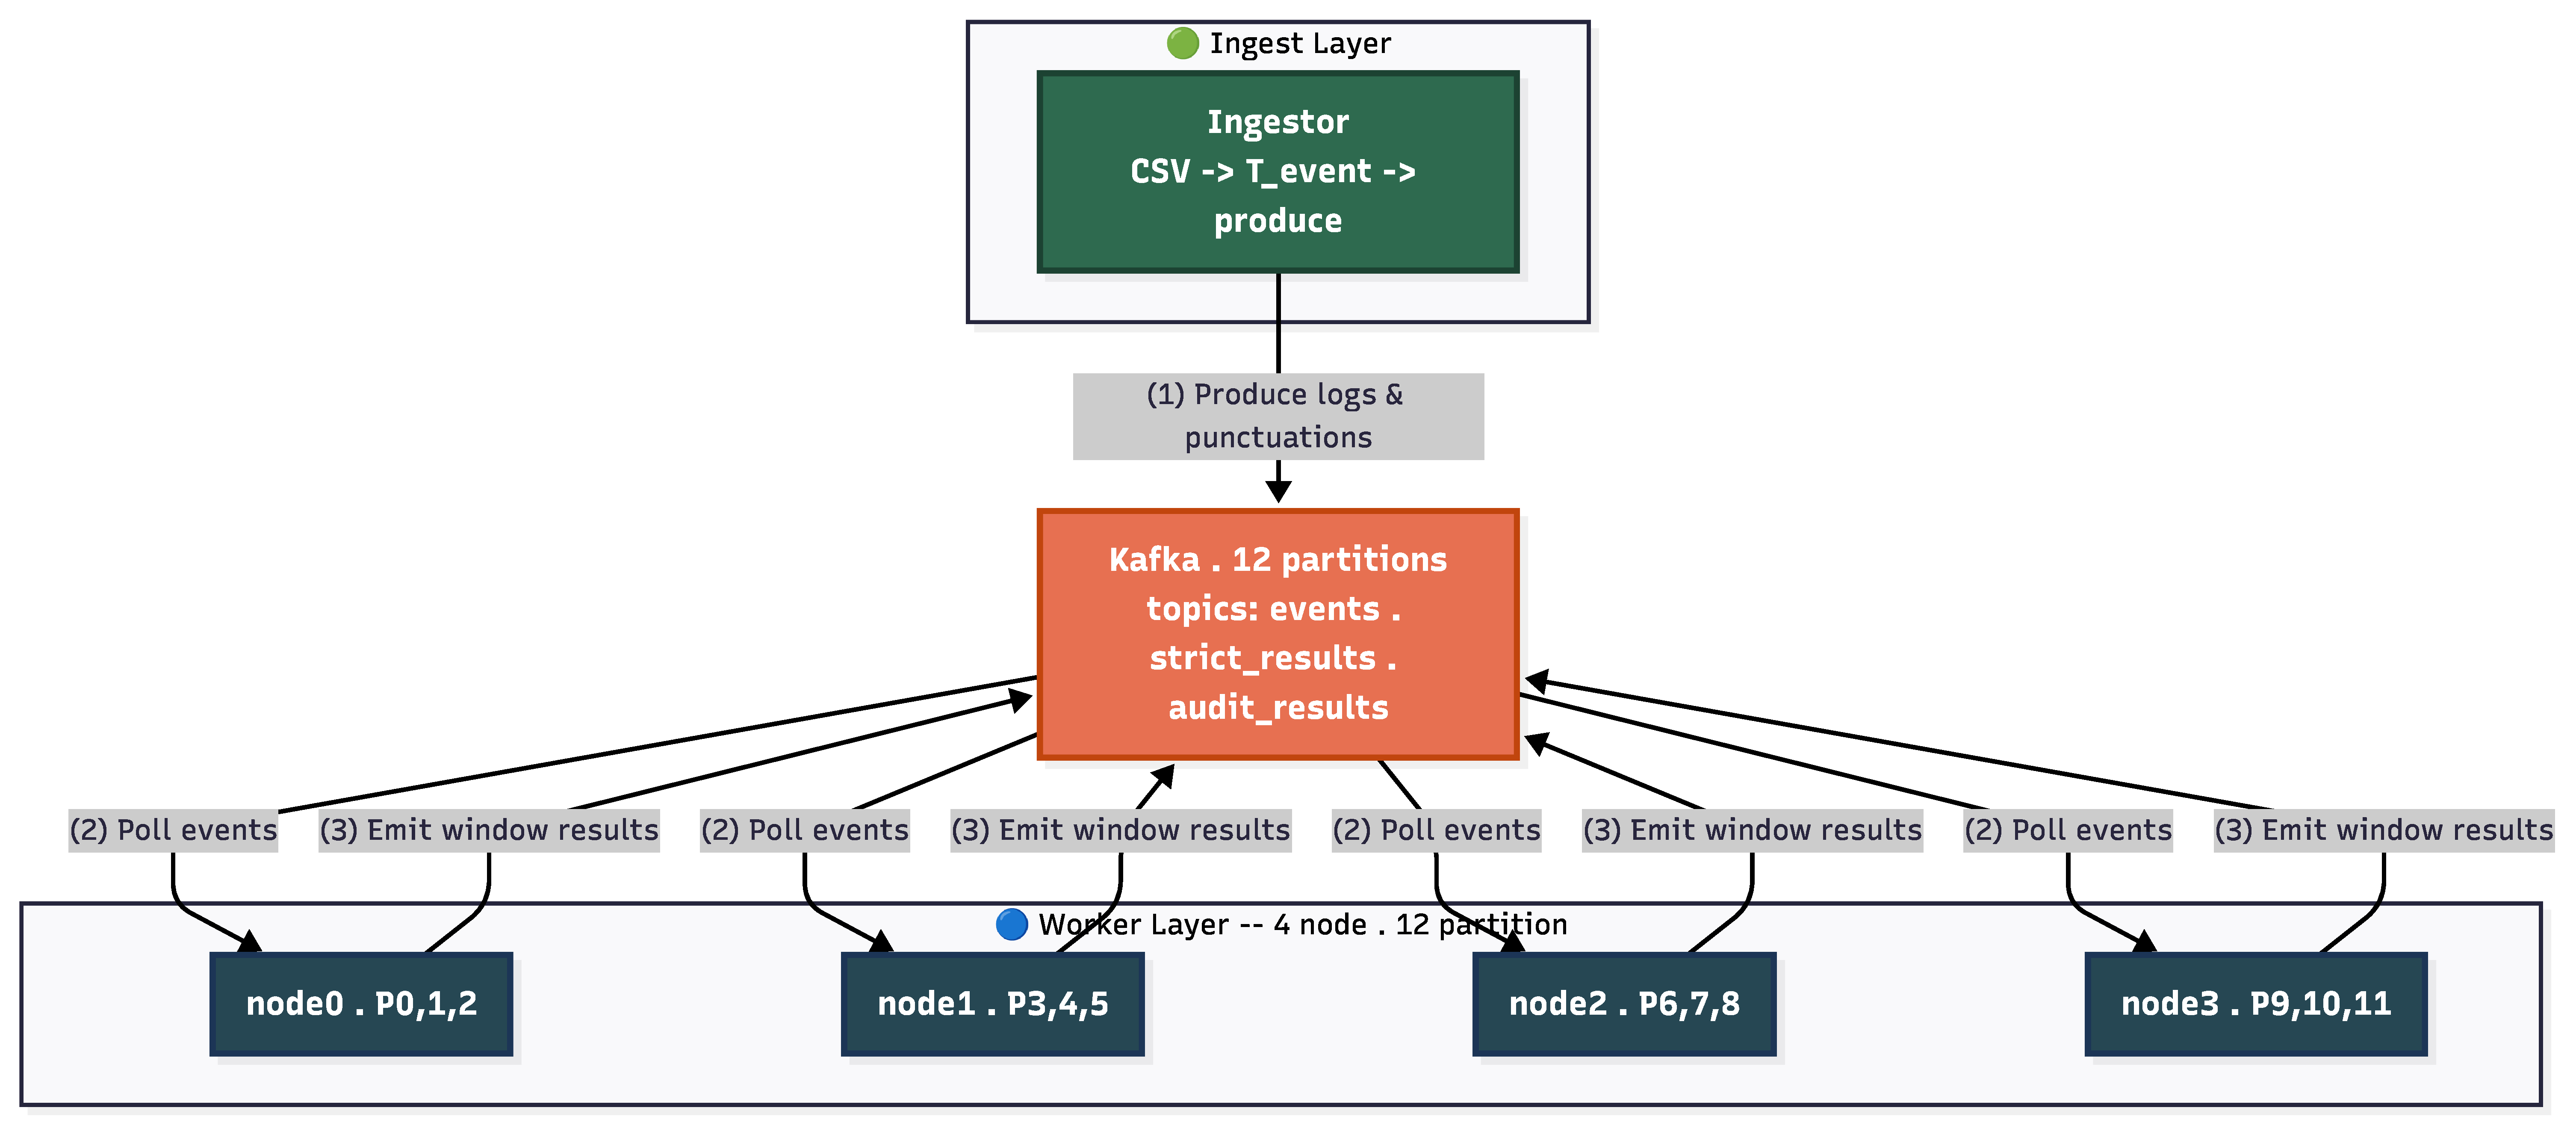
\includegraphics[width=\textwidth,height=10.0cm,keepaspectratio]{domain_4.1.pdf}
    \caption{Sơ đồ Domain 1: Luồng nạp dữ liệu từ Ingestor đến các Worker Nodes (Data Ingestion Domain).}
    \label{fig:domain1}
\end{figure}

\begin{table}[H]
    \centering
    \small
    \setlength{\tabcolsep}{4pt}
    \begin{tabular}{p{0.16\textwidth} p{0.21\textwidth} p{0.22\textwidth} p{0.29\textwidth}}
        \toprule
        \textbf{Luồng giao tiếp} & \textbf{Hướng} & \textbf{Giao thức / Cổng} & \textbf{Nội dung \& Tần suất} \\
        \midrule
        Produce log + punctuation & Ingestor $\to$ Kafka \texttt{events} & Kafka Producer (\texttt{acks=all}) & \texttt{LogEvent} (đã gán $T_{event}$) kèm Punctuation Token ($T_{commit}$); phân mảnh \texttt{hash(host)\%12}. Khi partition idle phát Empty Punctuation mỗi khoảng 1s (chỉ Strict). \\
        Poll events & Kafka \texttt{events} $\to$ Worker (N0--N3) & Kafka Consumer (pull) & Mỗi Worker poll partition được gán, nạp Bounded Min-Heap (sắp theo \texttt{event\_time}); backpressure \texttt{pause()}/\texttt{resume()} chống tràn RAM. \\
        Emit window results & Worker $\to$ Kafka \texttt{strict\_results} / \texttt{audit\_results} & Kafka Producer (\texttt{acks=all}) & Phát \texttt{WindowResult} khi $window\_end \le W$; idempotent theo \texttt{window\_id}; nhân bản song song sang Critical Audit Sink. \\
        \bottomrule
    \end{tabular}
    \caption{Chi tiết các luồng giao tiếp trong Domain 1 (Data Ingestion).}
\end{table}

\subsubsection{Domain 2: Luồng điều phối Strict Watermark (Strict Coordination Domain)}
Để cam kết bảo toàn dữ liệu tuyệt đối (0\% mất mát dữ liệu), luồng Strict Watermark duy trì cơ chế hội tụ toàn cục đồng thuận:
\begin{itemize}[leftmargin=*]
    \item \textbf{Local Watermark}: Các Worker Node nhận dữ liệu, tính toán Watermark cục bộ $LW_i(P_k)$ cho từng phân mảnh đang quản lý và gửi báo cáo thông qua luồng nhịp tim (heartbeat) về Coordinator.
    \item \textbf{High-Availability Coordinator Plane}: Cụm điều phối gồm 3 instance hoạt động theo thuật toán đồng thuận Raft (Leader-Follower). Coordinator Leader định kỳ tiếp nhận nhịp tim từ toàn bộ các Worker, tính toán Watermark toàn cục bằng giá trị nhỏ nhất của tất cả các phân mảnh hoạt động:
    {\large
    \begin{equation}
        \boxed{\displaystyle W_{global}(t) = \min_{\forall P_k \in \text{Active}} LW_i(P_k)}
    \end{equation}
    }
    Mốc Watermark toàn cục $W_{global}$ sau đó được broadcast ngược lại cho các Worker Nodes làm căn cứ chốt và giải phóng trạng thái cửa sổ.
\end{itemize}

Sơ đồ mô tả điều phối Strict:
\begin{figure}[H]
    \centering
    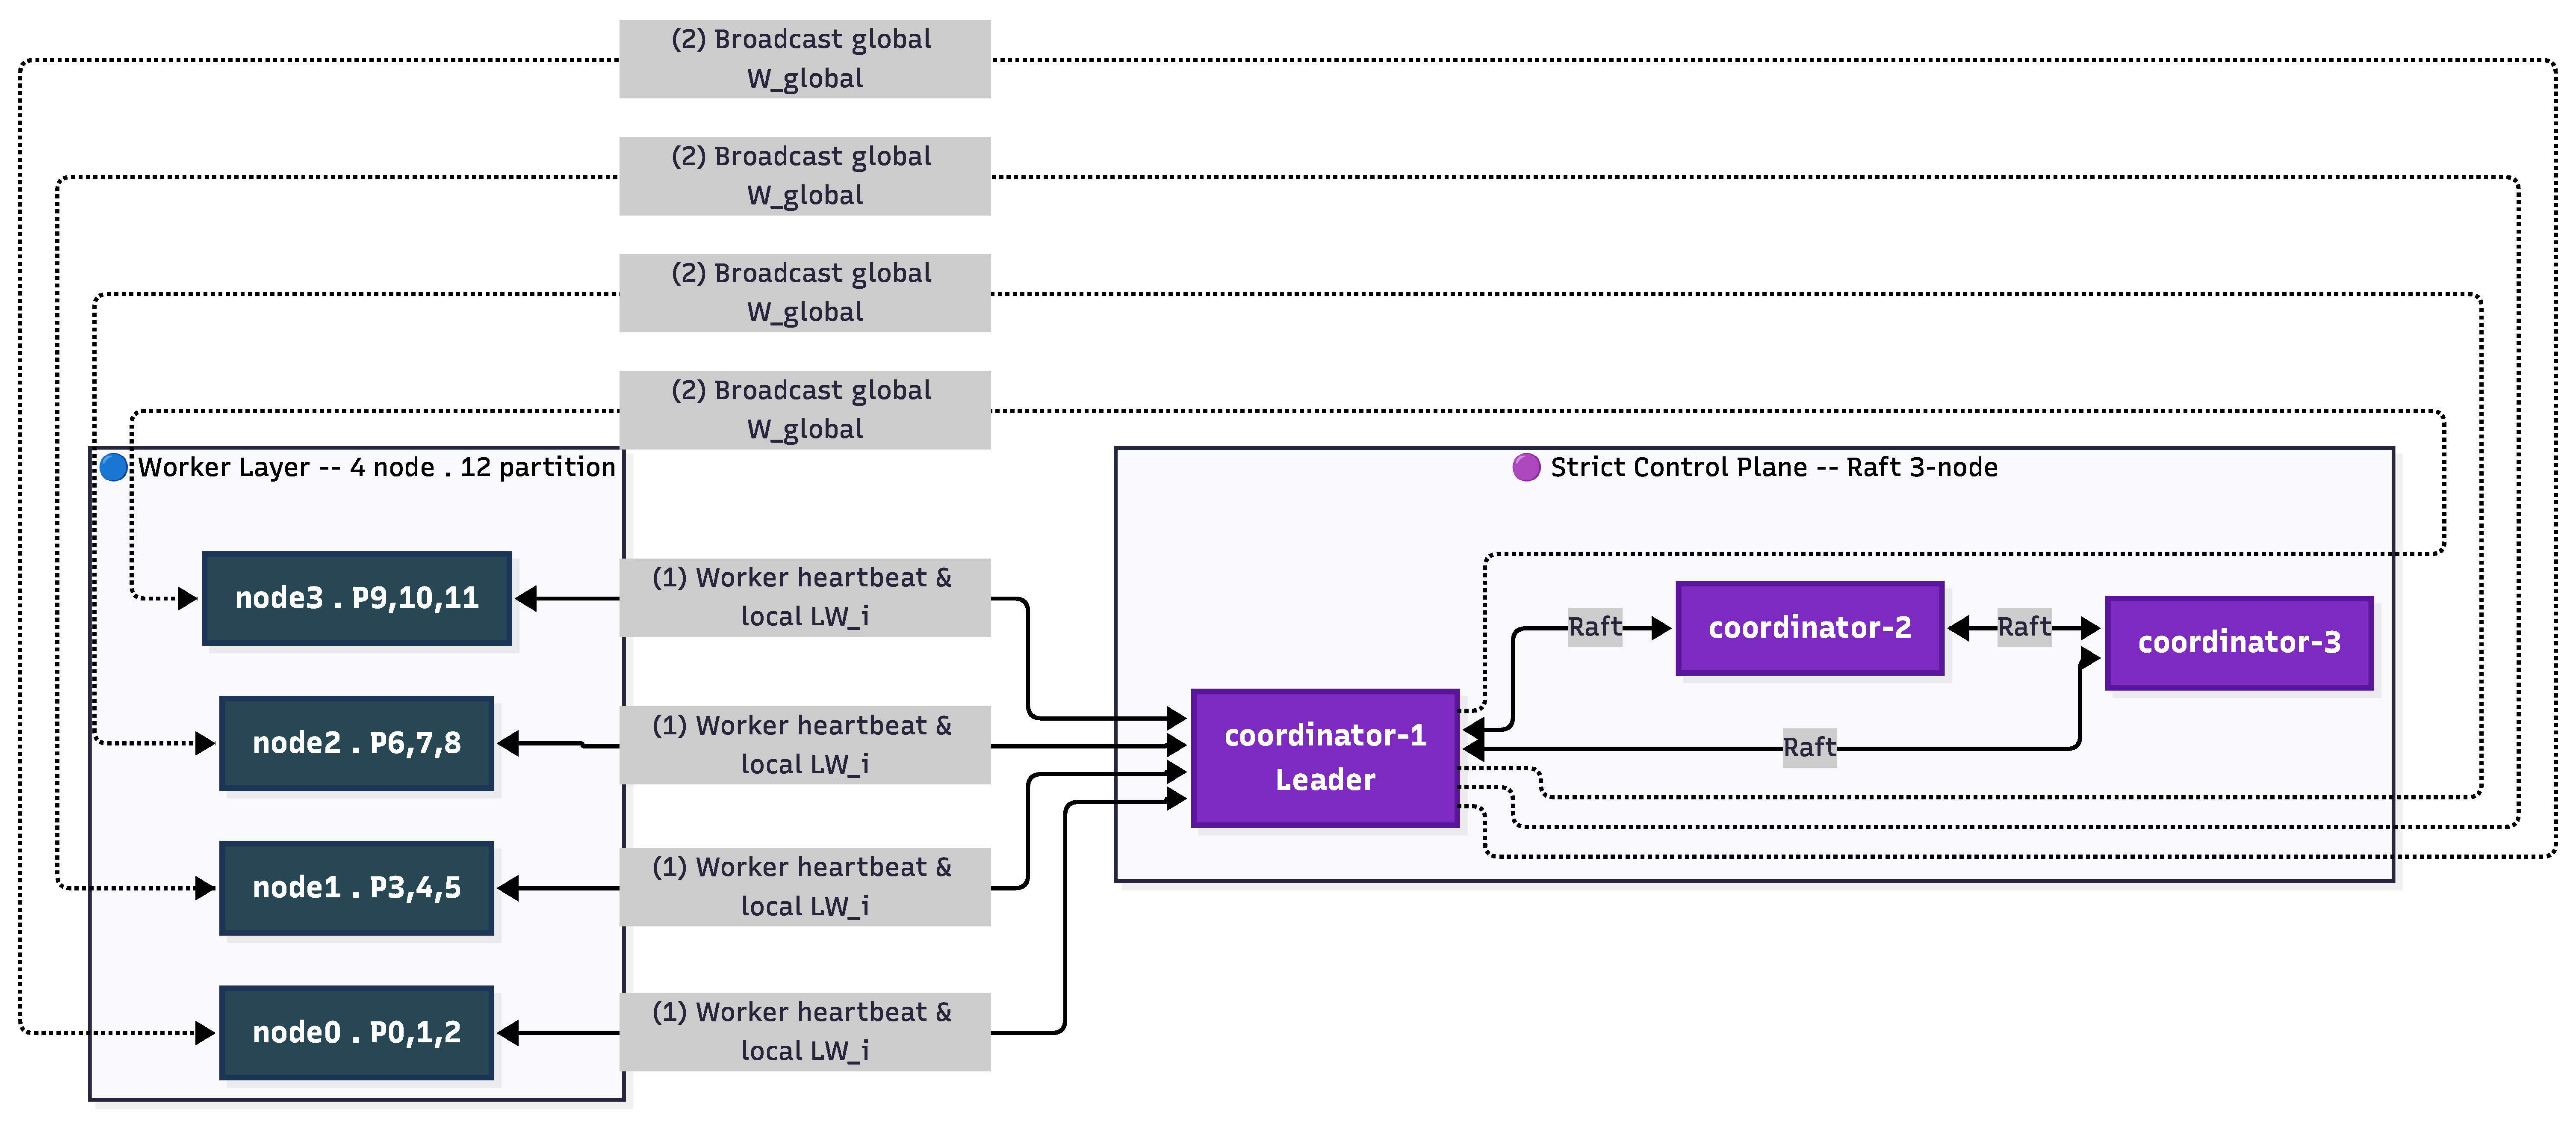
\includegraphics[width=\textwidth,height=10.0cm,keepaspectratio]{domain_4.2.pdf}
    \caption{Sơ đồ Domain 2: Luồng điều phối Strict Watermark (Strict Coordination Domain).}
    \label{fig:domain2}
\end{figure}

\begin{table}[H]
    \centering
    \small
    \setlength{\tabcolsep}{4pt}
    \begin{tabular}{p{0.16\textwidth} p{0.18\textwidth} p{0.27\textwidth} p{0.27\textwidth}}
        \toprule
        \textbf{Luồng giao tiếp} & \textbf{Hướng} & \textbf{Giao thức / Cổng} & \textbf{Nội dung \& Tần suất} \\
        \midrule
        Worker Heartbeat & Worker $\to$ Coordinator Leader & gRPC \texttt{WorkerHeartbeat} (cổng HTTP+50), fallback HTTP \texttt{POST /punctuation} & Bản đồ partition $\to$ \texttt{LW\_i}, kèm \texttt{max\_event\_time}, \texttt{kafka\_offsets}, \texttt{fencing\_token}, \texttt{idle\_partitions}; chu kỳ 1s. \\
        Get Global State & Worker $\to$ Coordinator Leader & gRPC \texttt{GetGlobalState}, fallback HTTP \texttt{GET /state} & Trả \texttt{W\_global}, \texttt{term}, \texttt{partition\_types}; Worker pull mỗi 500ms. \\
        Đồng thuận \& Bầu chọn HA & Leader $\leftrightarrow$ Followers / ZooKeeper & gRPC \texttt{RaftState}/\texttt{RaftVote} hoặc ZK Lock & Chế độ Raft: Sao chép \texttt{W\_global}, \texttt{partition\_assignment}, \texttt{term}; commit khi đa số (2/3) ack. Chế độ ZK: Leader sở hữu khóa tại \texttt{/csdlpt/coordinator-lock}, đồng bộ trạng thái qua gRPC/HTTP tới các follower. \\
        Failover / Failback & Coordinator $\to$ Worker & gRPC/HTTP kèm \texttt{(term, command\_id)} & Lệnh reassign / \texttt{PAUSE} / \texttt{RESUME} có fencing token; từ chối lệnh có \texttt{term} cũ. \\
        Broadcast \texttt{W\_global} & Coordinator (nội bộ) & Vòng lặp chủ động 200ms & Tính lại và đẩy \texttt{W\_global} + trạng thái partition phục vụ đồng bộ \& metrics. \\
        \bottomrule
    \end{tabular}
    \caption{Chi tiết các luồng giao tiếp trong Domain 2 (Strict Coordination).}
\end{table}

\subsubsection{Domain 3: Luồng điều phối Heuristic Watermark (Heuristic Aggregation Domain)}
Đối với chế độ tối ưu hóa độ trễ, luồng Heuristic Watermark sử dụng cấu trúc gom hợp thống kê bất đồng bộ:
\begin{itemize}[leftmargin=*]
    \item \textbf{Statistical Heartbeat}: Các Worker sử dụng cấu trúc dữ liệu DDSketch cục bộ để đo đạc độ trễ thực tế, báo cáo mốc Watermark thích ứng $W_h$ và bản chụp (snapshot) DDSketch cục bộ tới Aggregator.
    \item \textbf{Active-Standby Control Plane}: Cặp Aggregator dự phòng nóng (Primary-Standby). Việc tranh chấp Leader được thực hiện qua khóa phân tán ZooKeeper (\texttt{/csdlpt/aggregator-lock}) hoặc File Lock dùng chung (\texttt{FileLockLeader} hỗ trợ cross-platform \texttt{fcntl}/\texttt{msvcrt}). Standby liên tục theo dõi tệp nhịp tim của Active (\texttt{/tmp/aggregator-\{port\}-heartbeat} ghi mỗi 1s). Nếu nhịp tim mất hoặc quá hạn ($>1.5$\,s), Standby tự động chiếm khóa và được nâng lên làm Active, tải lại trạng thái phân mảnh và watermark từ RocksDB/JSON (\texttt{load\_state()}). Aggregator Active tổng hợp thông tin thu nhận để điều phối watermark thích ứng cục bộ, bản ghi muộn đi vào Dead-Letter Queue (DLQ).
\end{itemize}

Sơ đồ mô tả điều phối Heuristic:
\begin{figure}[H]
    \centering
    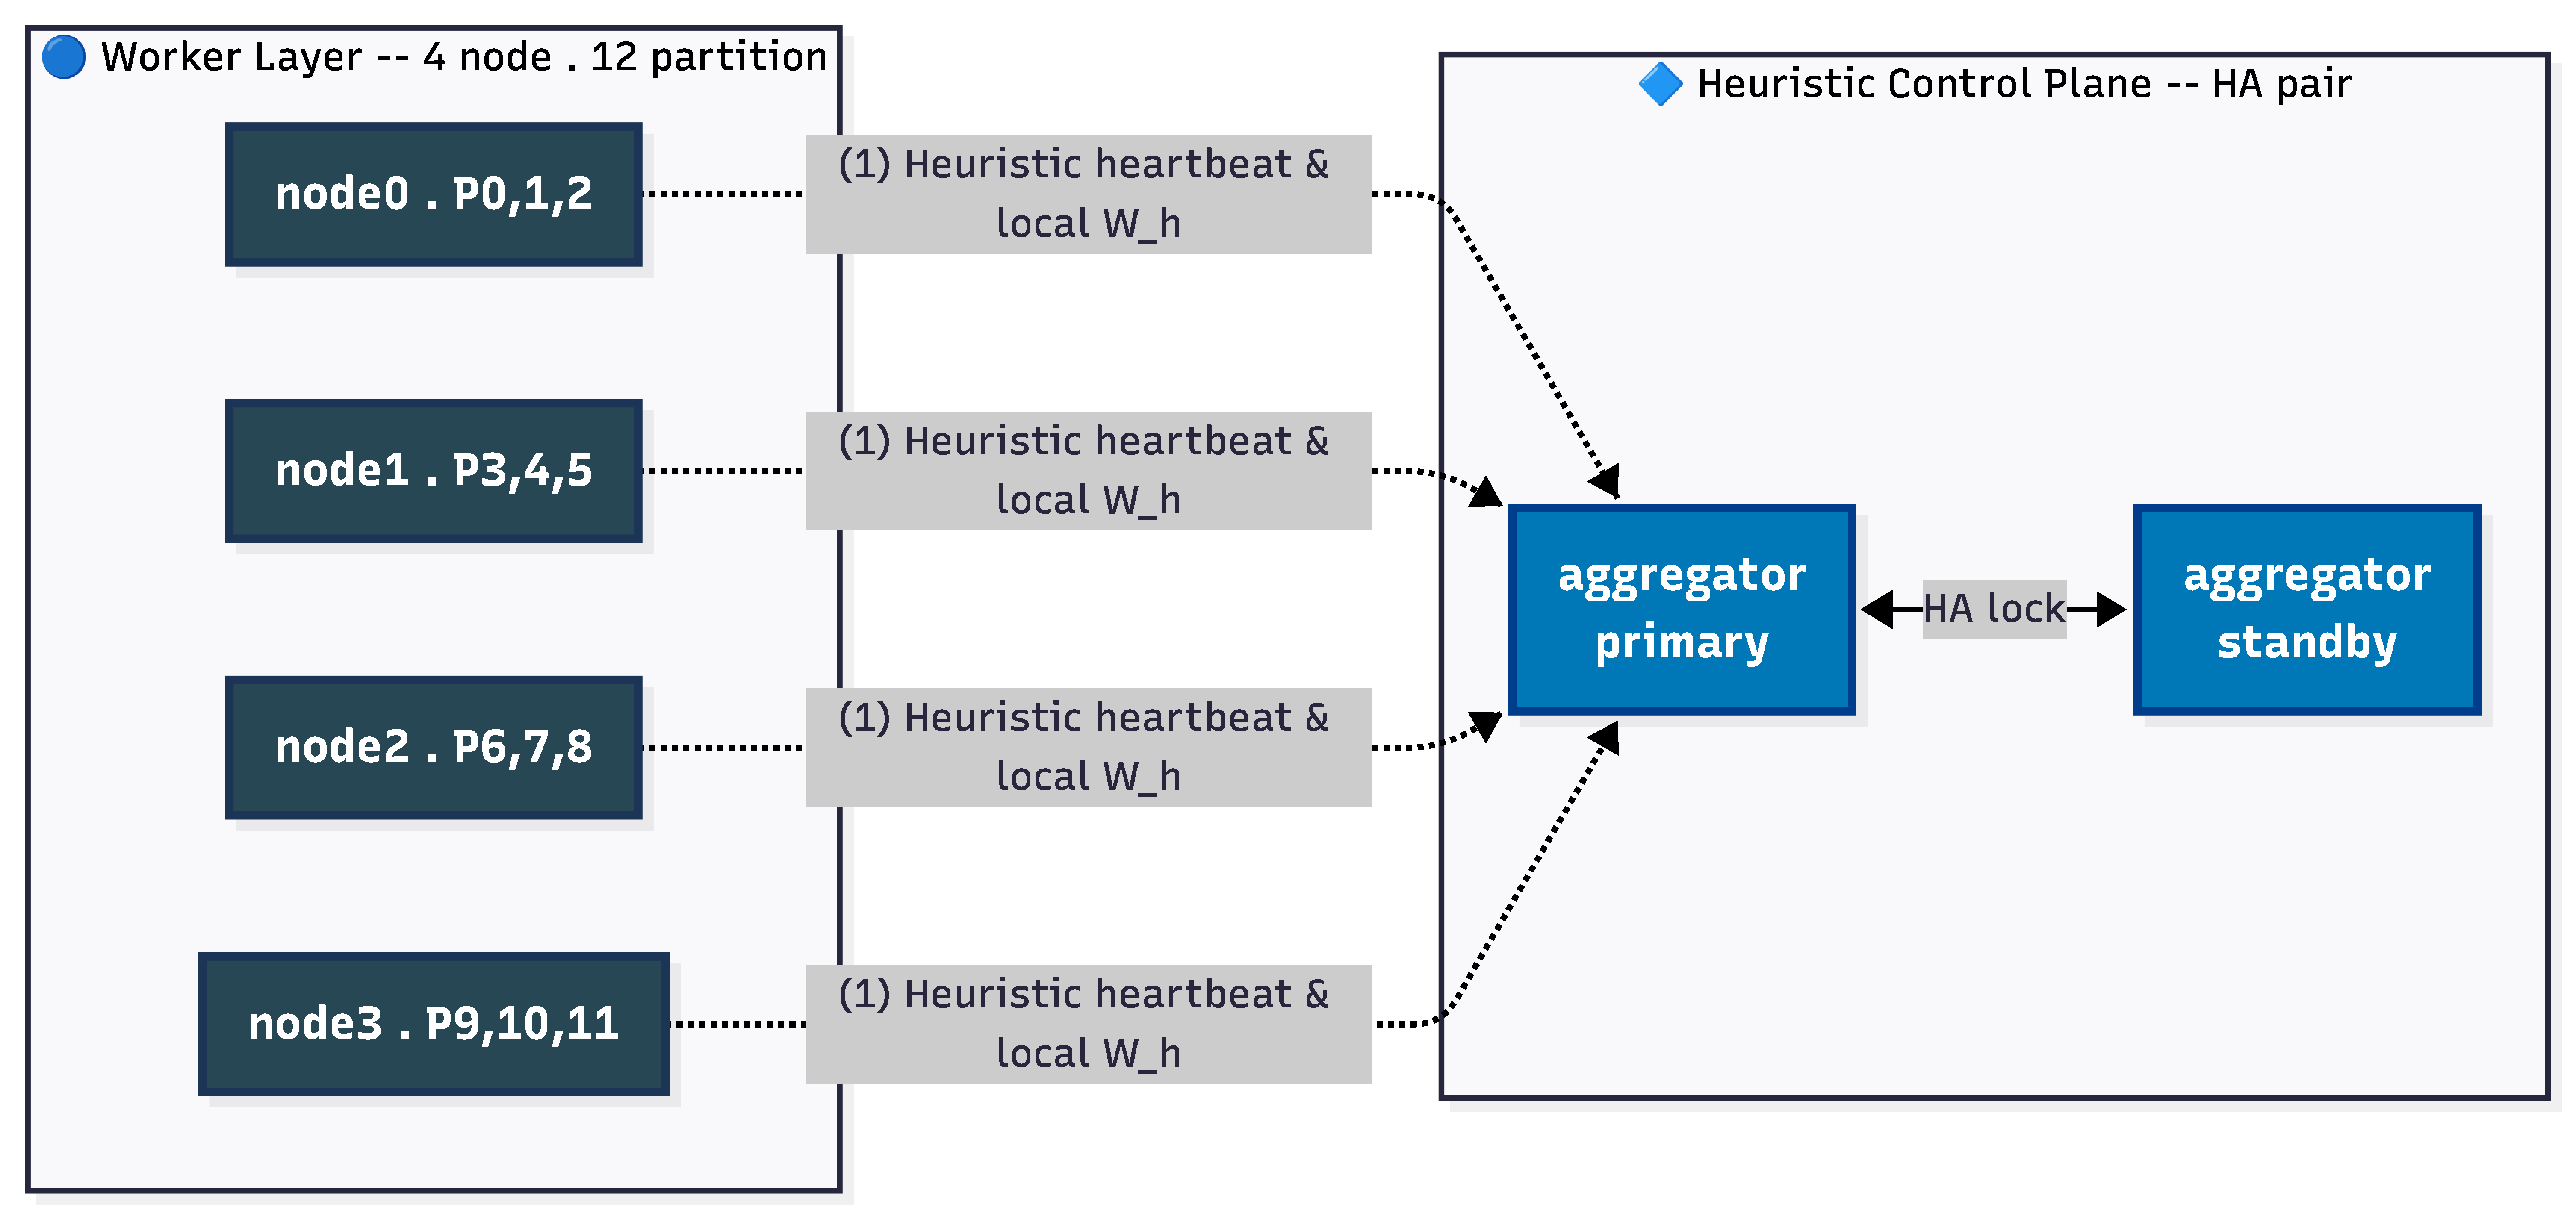
\includegraphics[width=\textwidth,height=10.0cm,keepaspectratio]{domain_4.3.pdf}
    \caption{Sơ đồ Domain 3: Luồng điều phối Heuristic Watermark (Heuristic Aggregation Domain).}
    \label{fig:domain3}
\end{figure}

\begin{table}[H]
    \centering
    \small
    \setlength{\tabcolsep}{4pt}
    \begin{tabular}{p{0.16\textwidth} p{0.18\textwidth} p{0.27\textwidth} p{0.27\textwidth}}
        \toprule
        \textbf{Luồng giao tiếp} & \textbf{Hướng} & \textbf{Giao thức / Cổng} & \textbf{Nội dung \& Tần suất} \\
        \midrule
        Heuristic Heartbeat & Worker $\to$ Aggregator Primary & gRPC \texttt{SendWorkerWatermark} (HTTP+50), fallback HTTP \texttt{POST /punctuation} & \texttt{worker\_id}, \texttt{partition\_id}, \texttt{W\_h} kèm \texttt{L\_eff} và snapshot DDSketch; chu kỳ khoảng 200ms. \\
        Tính watermark toàn cục & Aggregator (nội bộ) & Vòng lặp 500ms & $W_{global\_h} = \min(W_h)$ trên partition active; phân loại trạng thái \texttt{ACTIVE/STALE/IDLE/FAILED}. \\
        HA Active--Standby & Primary $\leftrightarrow$ Standby & Khóa ZooKeeper / File lock + Shared State & Standby theo dõi file nhịp tim ghi mỗi 1s. Mất nhịp tim $>$ 1.5s $\Rightarrow$ Standby chiếm khóa, khôi phục từ RocksDB/JSON và lên Active ($RTO\le 2$s). \\
        Broadcast \texttt{W\_global\_h} & Aggregator $\to$ Worker & HTTP \texttt{GET /state} (pull) & Worker nhận \texttt{W\_global\_h} thích ứng để chốt cửa sổ. \\
        Định tuyến dữ liệu muộn & Worker $\to$ Kafka \texttt{late\_logs\_dlq} & Kafka Producer & Sự kiện $T_{event} < W_h$ được đẩy DLQ; hạch toán \texttt{per\_window\_loss} thay vì chặn dòng chính. \\
        \bottomrule
    \end{tabular}
    \caption{Chi tiết các luồng giao tiếp trong Domain 3 (Heuristic Aggregation).}
\end{table}

\subsubsection{Domain 4: Phối hợp Control \& Metadata Plane (Control \& Infrastructure Domain)}
Mặt phẳng điều khiển và quản lý cấu hình hệ thống:
\begin{itemize}[leftmargin=*]
    \item \textbf{Ingestor Heartbeat}: Ingestor định kỳ gửi thông tin tiến độ đọc dữ liệu và độ lệch đồng hồ vật lý (\texttt{clock skew}) để Coordinator giám sát health và clock skew. Để tránh gRPC Fan-in Bottleneck, Ingestor đẩy heartbeat trực tiếp qua Kafka topic \texttt{ingestor-heartbeats}, sử dụng gRPC/HTTP làm luồng fallback.
    \item \textbf{Metadata Plane (ZooKeeper)}: ZooKeeper đóng vai trò trung tâm lưu trữ thông tin cấu hình cluster Kafka, thực hiện Service Discovery và hỗ trợ bầu chọn Leader cho các thành phần điều phối phân tán.
\end{itemize}

Sơ đồ mô tả Control \& Metadata Plane:
\begin{figure}[H]
    \centering
    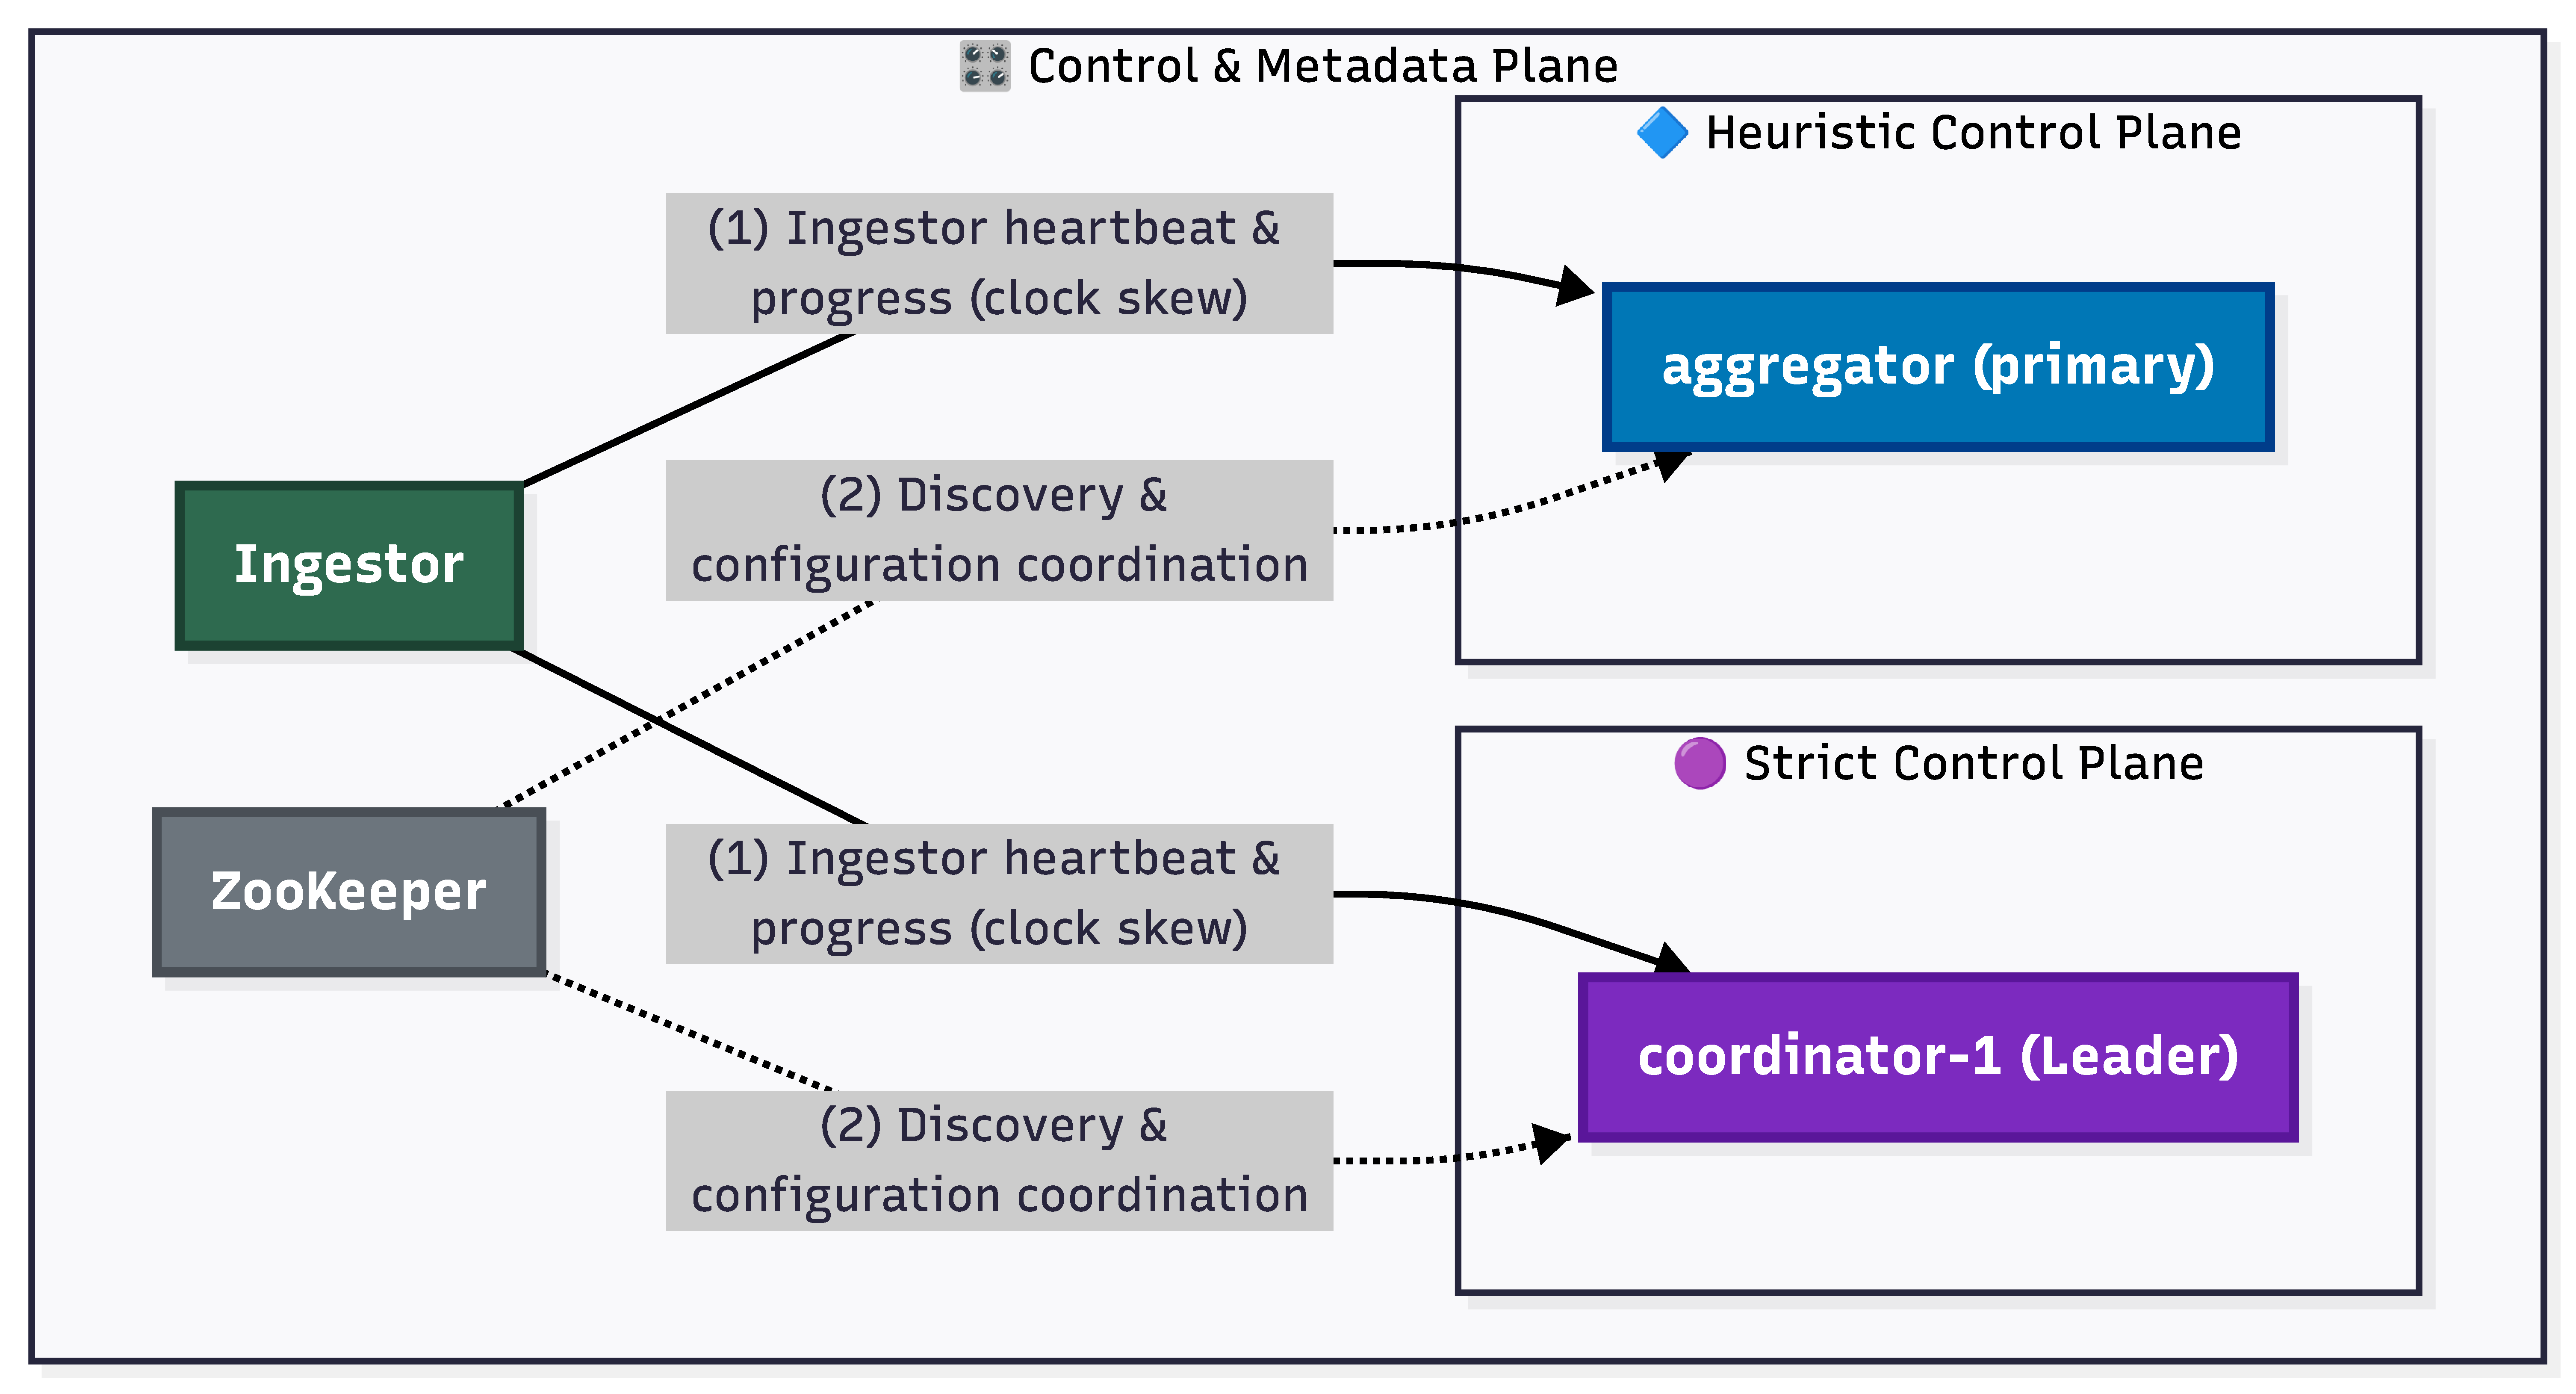
\includegraphics[width=\textwidth,height=10.0cm,keepaspectratio]{domain_4.4.pdf}
    \caption{Sơ đồ Domain 4: Phối hợp Control \& Metadata Plane (Control \& Infrastructure Domain).}
    \label{fig:domain4}
\end{figure}

\begin{table}[H]
    \centering
    \small
    \setlength{\tabcolsep}{4pt}
    \begin{tabular}{p{0.17\textwidth} p{0.20\textwidth} p{0.24\textwidth} p{0.27\textwidth}}
        \toprule
        \textbf{Luồng giao tiếp} & \textbf{Hướng} & \textbf{Giao thức / Cổng} & \textbf{Nội dung \& Tần suất} \\
        \midrule
        Ingestor Heartbeat & Ingestor $\to$ Kafka / Coordinator & Hàng đợi Kafka (\texttt{ingestor-heartbeats}) hoặc gRPC \texttt{IngestorHeartbeat} (fallback) & \texttt{ingestor\_id}, \texttt{T\_commit}, \texttt{timestamp}, \texttt{partitions\_assigned}, \texttt{ingestor\_clock}, \texttt{offsets}; gửi mỗi 5s; Coordinator nhận RTT để giám sát health và clock skew. \\
        Truy vấn giám sát & Dashboard / Ops $\to$ Coordinator \& Worker & HTTP \texttt{GET /health}, \texttt{/state}, \texttt{/api/metrics}, \texttt{/ingestor-health} & Bảng health/clock-skew, metrics completeness/latency, trạng thái \texttt{W\_global}/term/failover. \\
        Discovery \& cấu hình & ZooKeeper $\leftrightarrow$ Kafka / Coordinator / Aggregator & ZooKeeper & Lưu cấu hình cluster Kafka, bầu chọn Leader và hỗ trợ Service Discovery. \\
        \bottomrule
    \end{tabular}
    \caption{Chi tiết các luồng giao tiếp trong Domain 4 (Control \& Metadata).}
\end{table}

\subsubsection{Domain 5: Luồng lưu trữ trạng thái và Checkpoint (State \& Storage Domain)}
Cơ chế quản lý lưu trữ trạng thái phân tầng (Tiered State Storage) phục vụ mục tiêu khôi phục sau sự cố:
\begin{itemize}[leftmargin=*]
    \item \textbf{Tier-1 Hot State}: Mỗi Worker ghi nhận trạng thái cửa sổ đang mở trực tiếp vào RocksDB nhúng cục bộ trên SSD NVMe để đảm bảo độ trễ $<1$\,ms.
    \item \textbf{Tier-2 Warm State}: Định kỳ 10 giây, Worker sao lưu trạng thái xử lý logic và tệp dữ liệu RocksDB cục bộ sang Shared Volume chung phục vụ việc tiếp quản tức thời khi có node gặp sự cố.
    \item \textbf{Tier-3 Cold State}: Các kết quả cửa sổ đã chốt và dữ liệu lịch sử hoàn chỉnh được lưu trữ nén lâu dài trên Object Storage tương thích S3 (MinIO).
\end{itemize}

Sơ đồ mô tả lưu trữ và Checkpoint:
\begin{figure}[H]
    \centering
    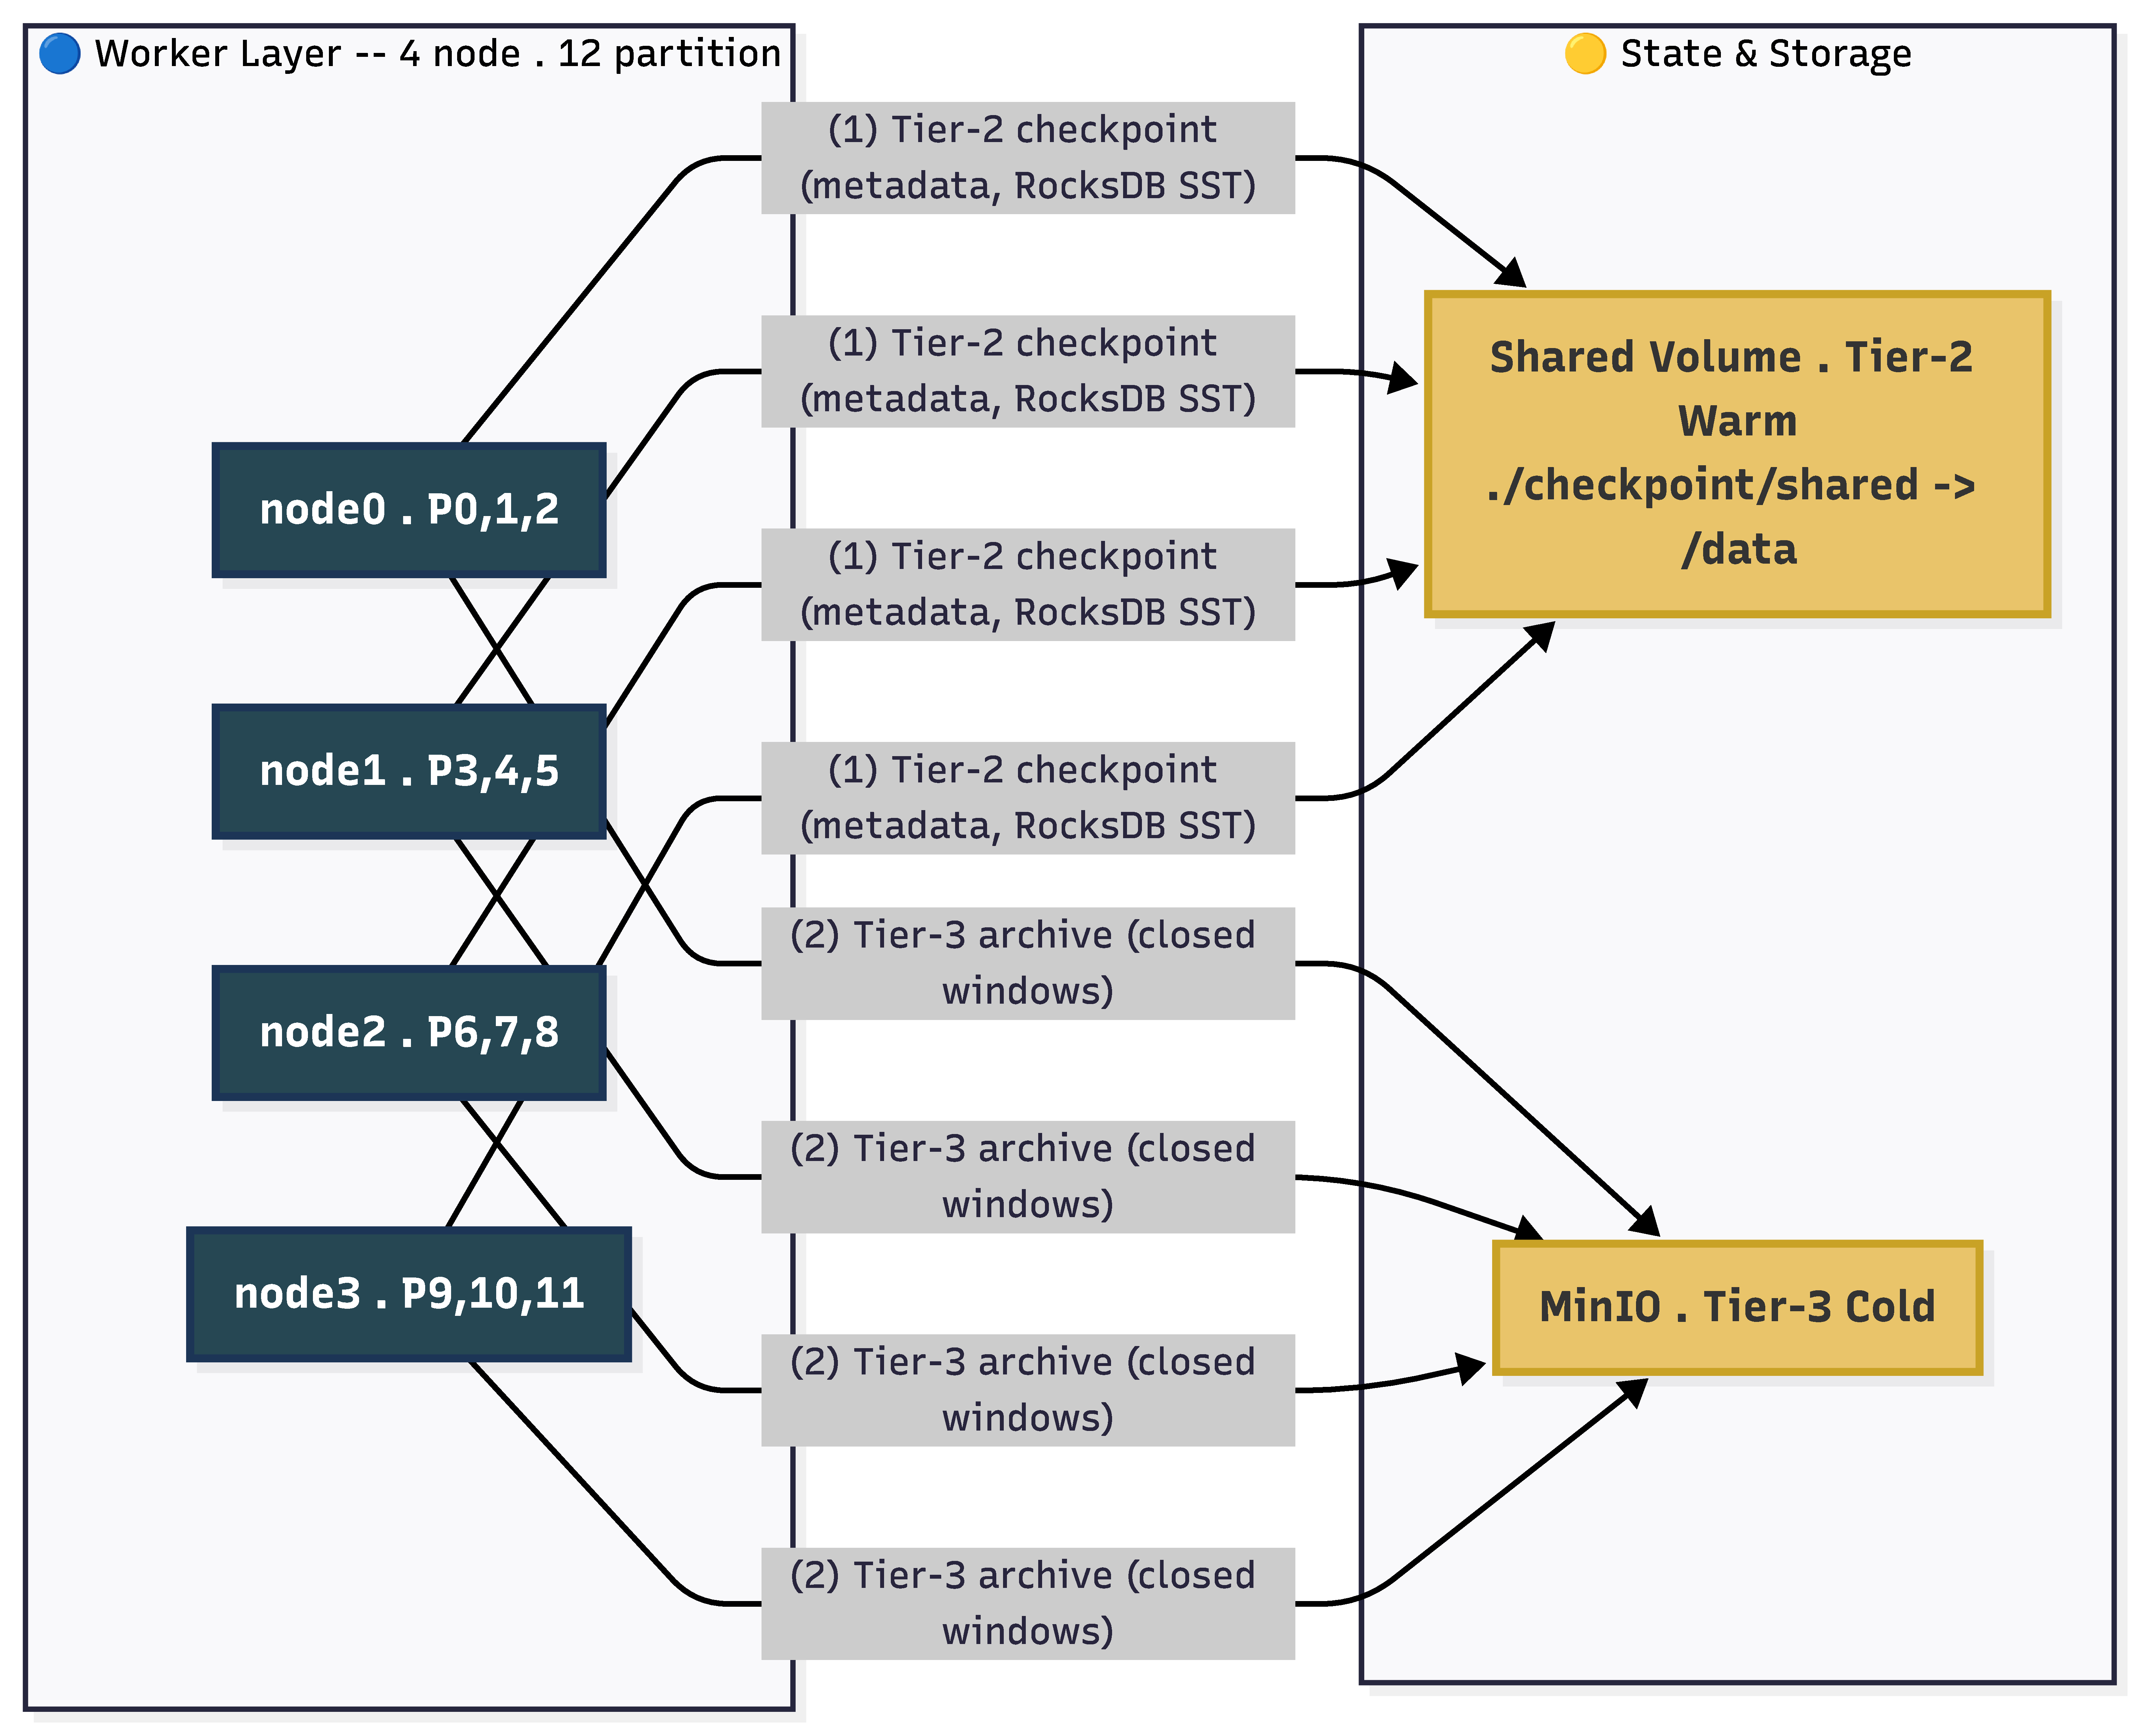
\includegraphics[width=\textwidth,height=10.0cm,keepaspectratio]{domain_4.5.pdf}
    \caption{Sơ đồ Domain 5: Luồng lưu trữ trạng thái và Checkpoint (State \& Storage Domain).}
    \label{fig:domain5}
\end{figure}

\begin{table}[H]
    \centering
    \small
    \setlength{\tabcolsep}{4pt}
    \begin{tabular}{p{0.15\textwidth} p{0.18\textwidth} p{0.24\textwidth} p{0.31\textwidth}}
        \toprule
        \textbf{Luồng giao tiếp} & \textbf{Hướng} & \textbf{Giao thức / Cổng} & \textbf{Nội dung \& Tần suất} \\
        \midrule
        Tier-1 Hot State & Worker $\leftrightarrow$ RocksDB cục bộ & RocksDB embedded (cô lập theo partition) & Đọc/ghi window state $<$ 1ms; namespace key \texttt{ow:} (open), \texttt{cw:} (closed), \texttt{si:} (seen-id dedupe), \texttt{meta:}. \\
        Tier-2 Checkpoint & Worker $\to$ Shared Volume & I/O file (\texttt{/data/checkpoint/partition\_\{pid\}/}) & Mỗi 10s ghi \texttt{checkpoint.json}, \texttt{emitted.json}, SST files + offset Kafka đã commit; phục vụ failover (node khác mount \& \texttt{seek(offset+1)}). \\
        Tier-3 Archive / DR & Worker $\to$ MinIO (S3) & MinIO client & Upload closed window theo key tất định \texttt{\{partition\}/\{window\_id\}.json}; eviction \texttt{CLOSED} $\to$ \texttt{UPLOADING} $\to$ \texttt{UPLOADED} $\to$ \texttt{PURGED}; backup active-state định kỳ (Disaster Recovery). \\
        \bottomrule
    \end{tabular}
    \caption{Chi tiết các luồng giao tiếp trong Domain 5 (State \& Storage).}
\end{table}

\subsection{Vai trò của các thành phần trong hệ thống (Container View)}
Dưới đây là chi tiết vai trò của các thực thể trong kiến trúc hệ thống xử lý luồng Watermark phân tán:

\begin{longtable}{p{0.18\textwidth} p{0.22\textwidth} p{0.50\textwidth}}
\toprule
\textbf{Ký hiệu Node} & \textbf{Phân lớp (Layer)} & \textbf{Mô tả vai trò \& Chức năng chính} \\
\midrule
\endhead
\texttt{ING} & Ingestor & Đọc dữ liệu CSV từ thư mục chia sẻ, gán nhãn thời gian sự kiện ($T_{event}$), gửi dữ liệu và Punctuation Token vào Kafka. \\
\texttt{KAFKA} & Data Plane & Broker điều phối thông điệp, lưu trữ các phân vùng (12 partitions) của các topic (events, strict\_results, audit\_results). \\
\texttt{ZK} & Auxiliary & Quản lý cấu hình cluster Kafka, hỗ trợ bầu chọn Leader (Coordinator/Aggregator) và phát hiện dịch vụ (Service Discovery). \\
\texttt{N0} -- \texttt{N3} & Worker Layer & Các thực thể tính toán chạy song song, tiêu thụ dữ liệu từ các partition Kafka được phân bổ, quản lý window và tính toán Watermark cục bộ. \\
\texttt{C1} -- \texttt{C3} & Strict Control Plane & Cụm điều phối trạng thái hoạt động theo giải thuật đồng thuận Raft (Leader-Follower) để tính toán Watermark toàn cục ($W_{global}$) trong chế độ Strict. \\
\texttt{AGG} / \texttt{AGGS} & Heuristic Control Plane & Cặp cấu hình dự phòng nóng (HA qua khóa phân tán) để thu thập dữ liệu thống kê từ Workers và điều phối Watermark toàn cục trong chế độ Heuristic. \\
\texttt{VOL} & Storage (Tier-2) & Phân vùng lưu trữ chia sẻ cục bộ, lưu checkpoint trạng thái (mỗi 10s) của các worker để hỗ trợ Failover tức thời. \\
\texttt{MINIO} & Storage (Tier-3) & Kho lưu trữ đối tượng dạng S3 tương thích, lưu trữ lâu dài các kết quả của các window đã được chốt (Purged/Closed). \\
\texttt{DASH} & Streamlit UI & Giao diện người dùng đồ họa để theo dõi hiệu năng hệ thống (completeness vs wait time), gửi lệnh Docker Compose điều khiển bật/tắt các container. \\
\bottomrule
\caption{Bảng đặc tả chi tiết vai trò các thành phần cấu trúc hệ thống.}
\end{longtable}

\subsection{Vai trò của các tiến trình trong mã nguồn (Executable Processes)}
Các vai trò tiến trình tương ứng được định nghĩa trong tệp mã nguồn \texttt{run.py} thông qua các đối số dòng lệnh:

\begin{longtable}{p{0.22\textwidth} p{0.28\textwidth} p{0.44\textwidth}}
\toprule
\textbf{Vai trò (Role)} & \textbf{Lệnh dòng lệnh tương ứng} & \textbf{Mô tả chức năng mã nguồn} \\
\midrule
\endhead
\texttt{ingestor} & \texttt{--role ingestor} & Đọc CSV trong \texttt{/dataset}, gán \texttt{T\_event}, produce log + Punctuation Token vào Kafka. \\
\texttt{worker} & \texttt{--role worker} & Poll Kafka, sort theo event-time (Bounded PQ), dedupe, gom window, ghi RocksDB, emit kết quả. \\
\texttt{coordinator} & \texttt{--role coordinator} & Cụm 3 node Raft. Tính $W_{global} = \min(LW_i)$, điều phối failover, fencing token. \\
\texttt{aggregator} & \texttt{--role aggregator} & Primary + standby (HA qua lock). Tổng hợp $W_{global\_h}$ từ DDSketch của worker. \\
\bottomrule
\caption{Bảng đặc tả các tiến trình thực thi của hệ thống.}
\end{longtable}

\subsection{Hợp đồng giao tiếp giữa các Domain và Giải pháp cho bài toán nút cổ chai (Stragglers)}

Để hệ thống hoạt động đồng bộ và bền vững, các giao tiếp giữa các Domain được chuẩn hóa thành các hợp đồng dịch vụ (Service Contracts) chặt chẽ:
\begin{enumerate}
    \item \textbf{Hợp đồng Ingestion (Data Ingestion Contract)}: Ingestor cam kết phân mảnh dữ liệu hành trình xe taxi ngang theo hàm băm và gán thời gian sự kiện logic $T_{event}$. Trong chế độ nghiêm ngặt (Strict), Ingestor phải phát thông điệp kiểm soát (Punctuation Token) chứa mốc cam kết $T_{commit}$. Khi một phân mảnh không có chuyến đi mới phát sinh (nhàn rỗi), Ingestor định kỳ gửi các \textit{Empty Punctuation Token} với $T_{commit}$ tăng dần để dòng chảy thời gian của phân mảnh đó không bị dừng.
    \item \textbf{Hợp đồng Heartbeat của Worker (Worker Heartbeat Contract)}: Định kỳ 1 giây, các Worker gửi báo cáo trạng thái qua gRPC \texttt{WorkerHeartbeat} tới Coordinator. Nội dung báo cáo bao gồm: mốc thời gian Watermark cục bộ của từng phân mảnh đang quản lý $LW_i(P_k)$, offset Kafka đã xử lý, và danh sách các phân mảnh bị nhàn rỗi (\texttt{idle\_partitions}).
    \item \textbf{Hợp đồng Trạng thái Toàn cục (Global State Contract)}: Các Worker định kỳ 500 ms truy vấn Coordinator qua gRPC \texttt{GetGlobalState} để nhận mốc thời gian Watermark toàn cục $W_{global}$ phục vụ cho việc chốt và giải phóng trạng thái cửa sổ thời gian logic.
\end{enumerate}

\subsubsection{Cơ chế giải quyết bài toán nút cổ chai (Stragglers)}

Hiện tượng nút cổ chai xảy ra khi một hoặc một vài phân mảnh bị xử lý chậm trễ hoặc không có dữ liệu phát sinh (Idle Partition), kéo mốc Watermark toàn cục dừng lại và làm tràn bộ nhớ đệm trạng thái RAM (MemTable) tại tất cả các Worker khác. Hệ thống giải quyết bài toán này qua hai chiến lược chuyên biệt:

\paragraph{Giải pháp trong chế độ Strict (Empty Punctuation \& Idleness Bypass):}
\begin{itemize}[label={-}]
    \item Khi Worker nhận được Empty Punctuation Token từ Kafka, nó sẽ tịnh tiến watermark cục bộ $LW_i(P_k)$ của phân mảnh đó lên.
    \item Nếu một phân mảnh nhàn rỗi quá thời gian quy định (\texttt{IDLE\_TIMEOUT\_S}), Worker sẽ tự động đánh dấu phân mảnh đó là \texttt{TEMPORARY\_IDLE} và gửi báo cáo danh sách này lên Coordinator.
    \item Coordinator Leader khi tính toán watermark toàn cục theo công thức hội tụ tối thiểu \emph{đơn điệu}:
    {\large
    \begin{equation}
        \boxed{\displaystyle W_{global}(t) = \max\Big(W_{global}^{prev},\ \min_{P_k \notin \text{Idle}} LW_i(P_k)\Big)}
    \end{equation}
    }
    Sẽ tạm thời loại trừ các phân mảnh nhàn rỗi tường minh ra khỏi hàm $\min$, cho phép $W_{global}$ tiếp tục tiến lên, giải phóng trạng thái cửa sổ của các phân mảnh hoạt động khác. Khi phân mảnh nhàn rỗi có dữ liệu trở lại, nó sẽ tự động được đưa trở lại danh sách tính toán.
    \item \textbf{Lưu ý đồng bộ mã hiện thực} (\texttt{strict/coordinator.py}): Empty Punctuation là cơ chế \emph{chính} giữ $W_{global}$ tịnh tiến nên hệ thống \textbf{không} loại bỏ ngầm các phân mảnh chỉ vì im lặng. Các phân mảnh phản hồi chậm (\texttt{STALE}) và nhàn rỗi ngầm (\texttt{IDLE}) vẫn nằm trong hàm $\min()$; chỉ phân mảnh xác nhận lỗi (\texttt{FAILED}) hoặc được Worker đánh dấu \texttt{is\_temporary\_idle} mới bị loại trừ, bảo toàn cam kết 0\% loss.
\end{itemize}

Sơ đồ trình tự xử lý phân mảnh nhàn rỗi bằng Empty Punctuation trong chế độ Strict:
\begin{figure}[H]
    \centering
    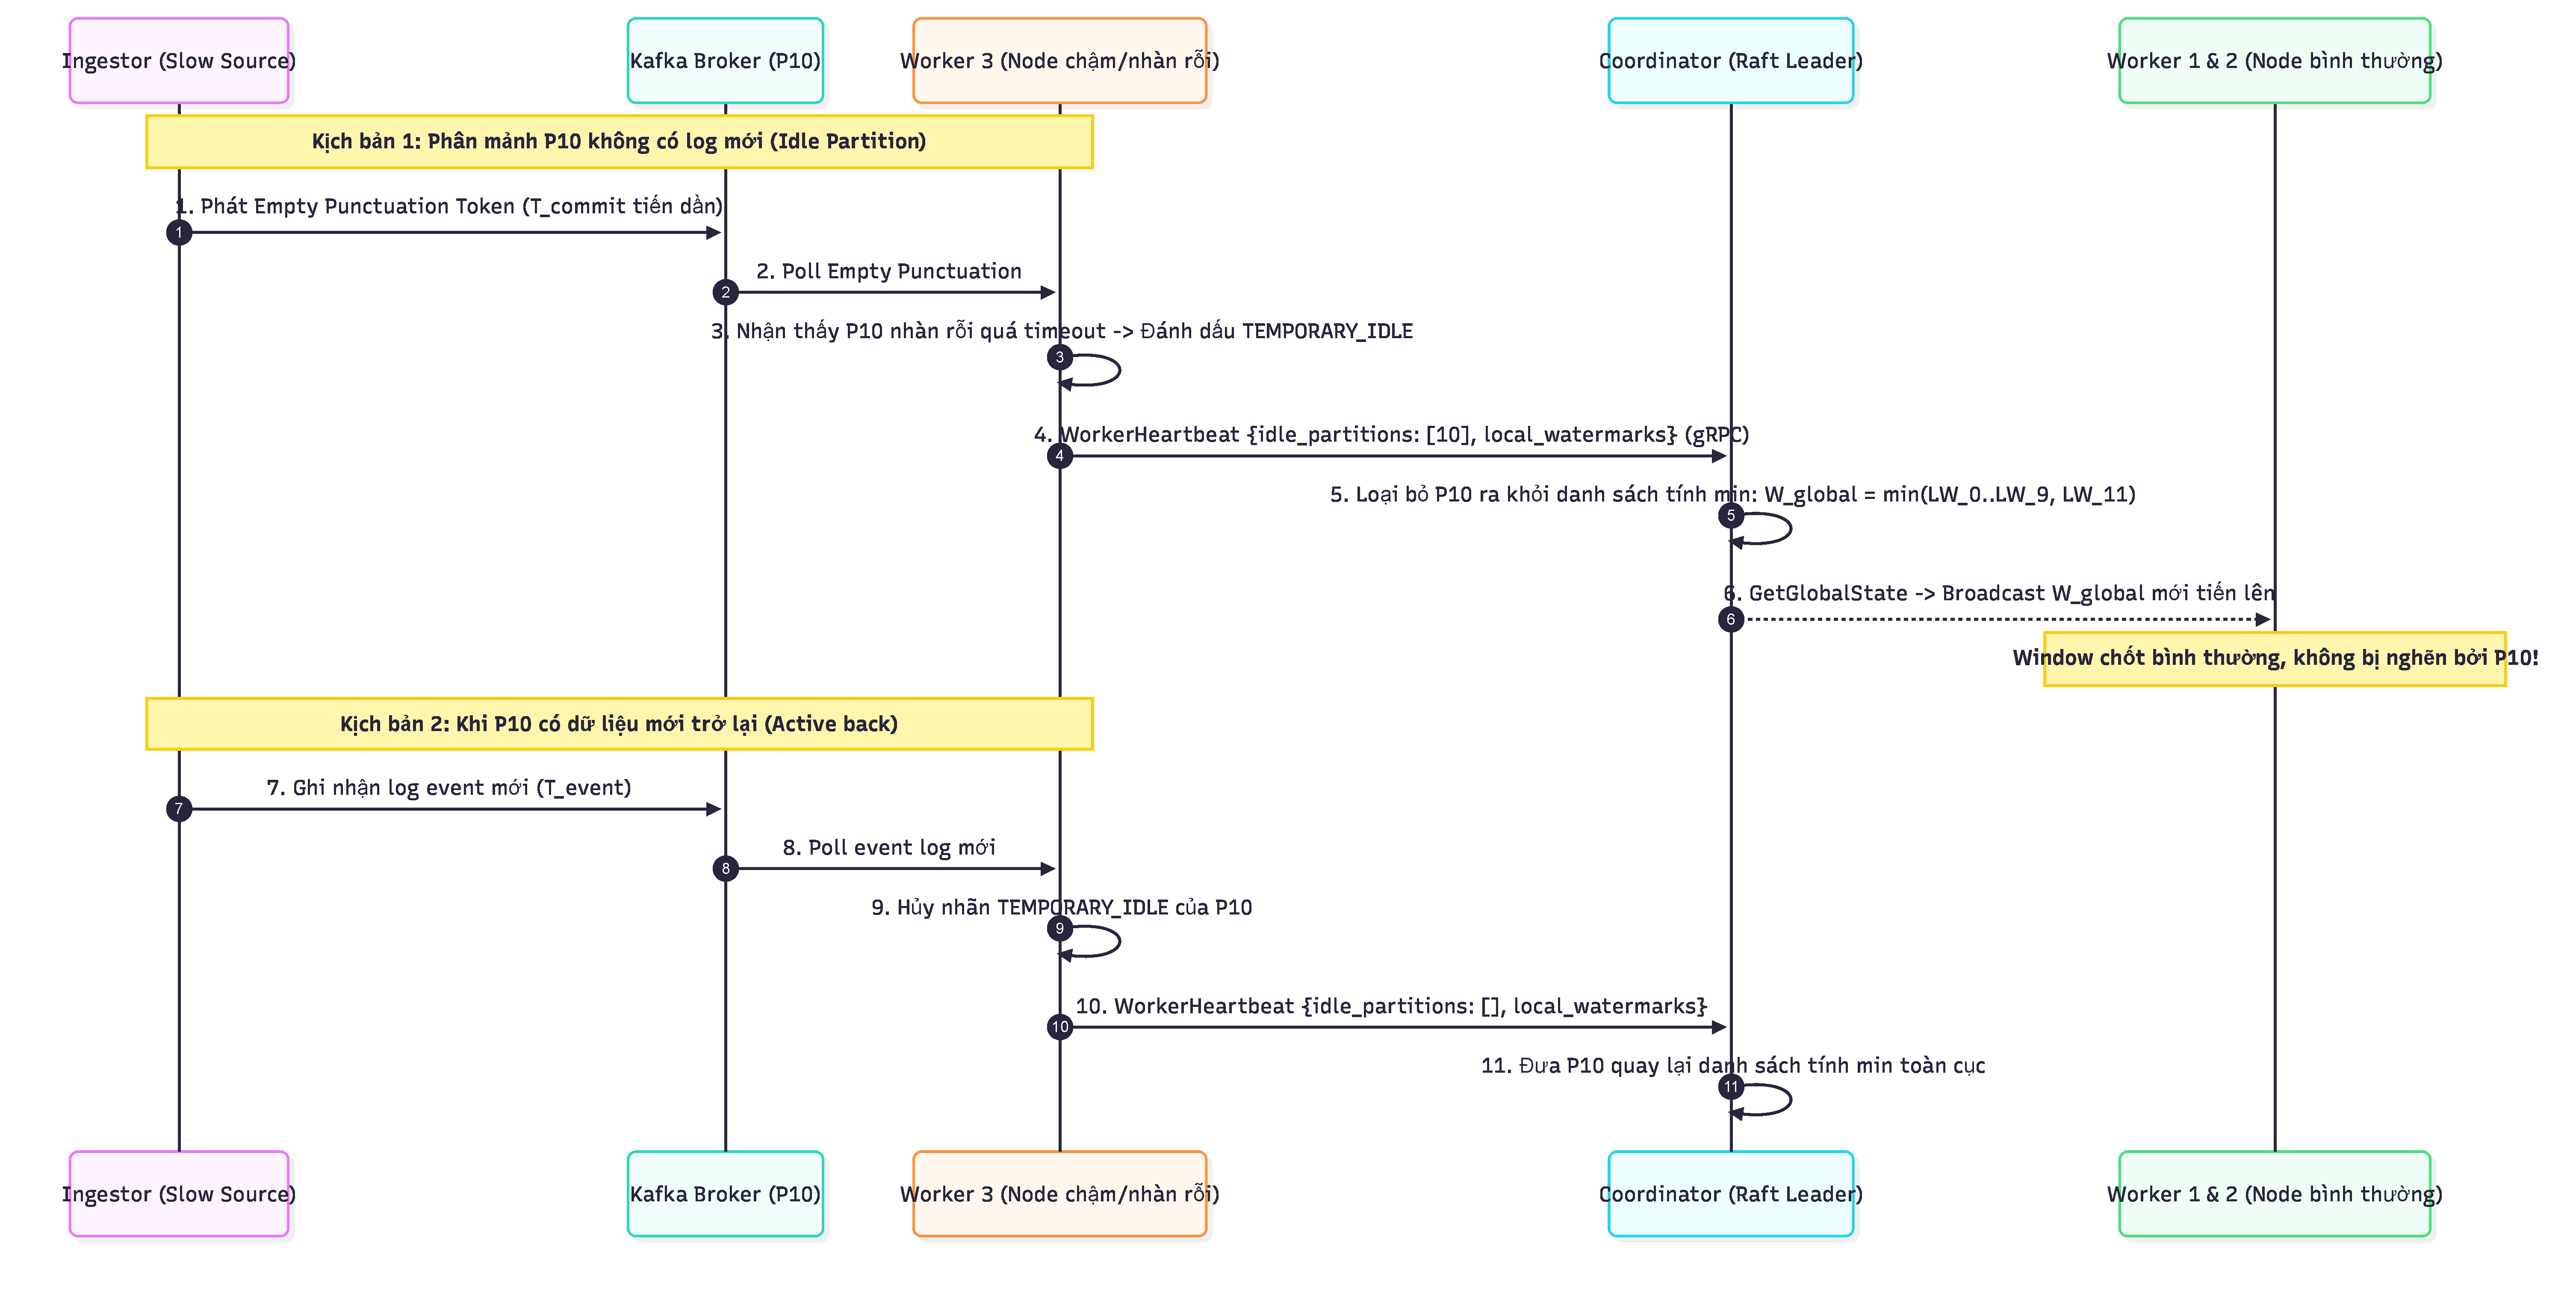
\includegraphics[width=\textwidth,height=15.0cm,keepaspectratio]{Empty Punctuation.pdf}
    \caption{Trình tự xử lý Straggler chế độ Strict: Empty Punctuation \& Idleness Bypass.}
    \label{fig:emptypunctuation}
\end{figure}

\paragraph{Giải pháp trong chế độ Heuristic (DDSketch \& DLQ routing):}
\begin{itemize}[label={-}]
    \item Không có sự phụ thuộc toàn cục. Mỗi Worker tự ước lượng phân phối độ trễ cục bộ của phân mảnh đang giữ bằng cấu trúc dữ liệu DDSketch và tự xác định mốc chốt cửa sổ thích ứng $W_h$ mà không cần chờ đợi các phân mảnh khác.
    \item Nếu một phân mảnh bị chậm (Straggler), các sự kiện đến muộn sau khi cửa sổ đã chốt sẽ không làm tắc nghẽn luồng xử lý chính. Chúng sẽ được định tuyến tự động vào Hàng đợi xử lý muộn (Dead-Letter Queue - DLQ) để xử lý đền bù trạng thái lịch sử sau đó, đảm bảo độ trễ chốt cửa sổ luôn ở mức tối thiểu.
\end{itemize}

Sơ đồ trình tự định tuyến dữ liệu muộn sang DLQ trong chế độ Heuristic:
\begin{figure}[H]
    \centering
    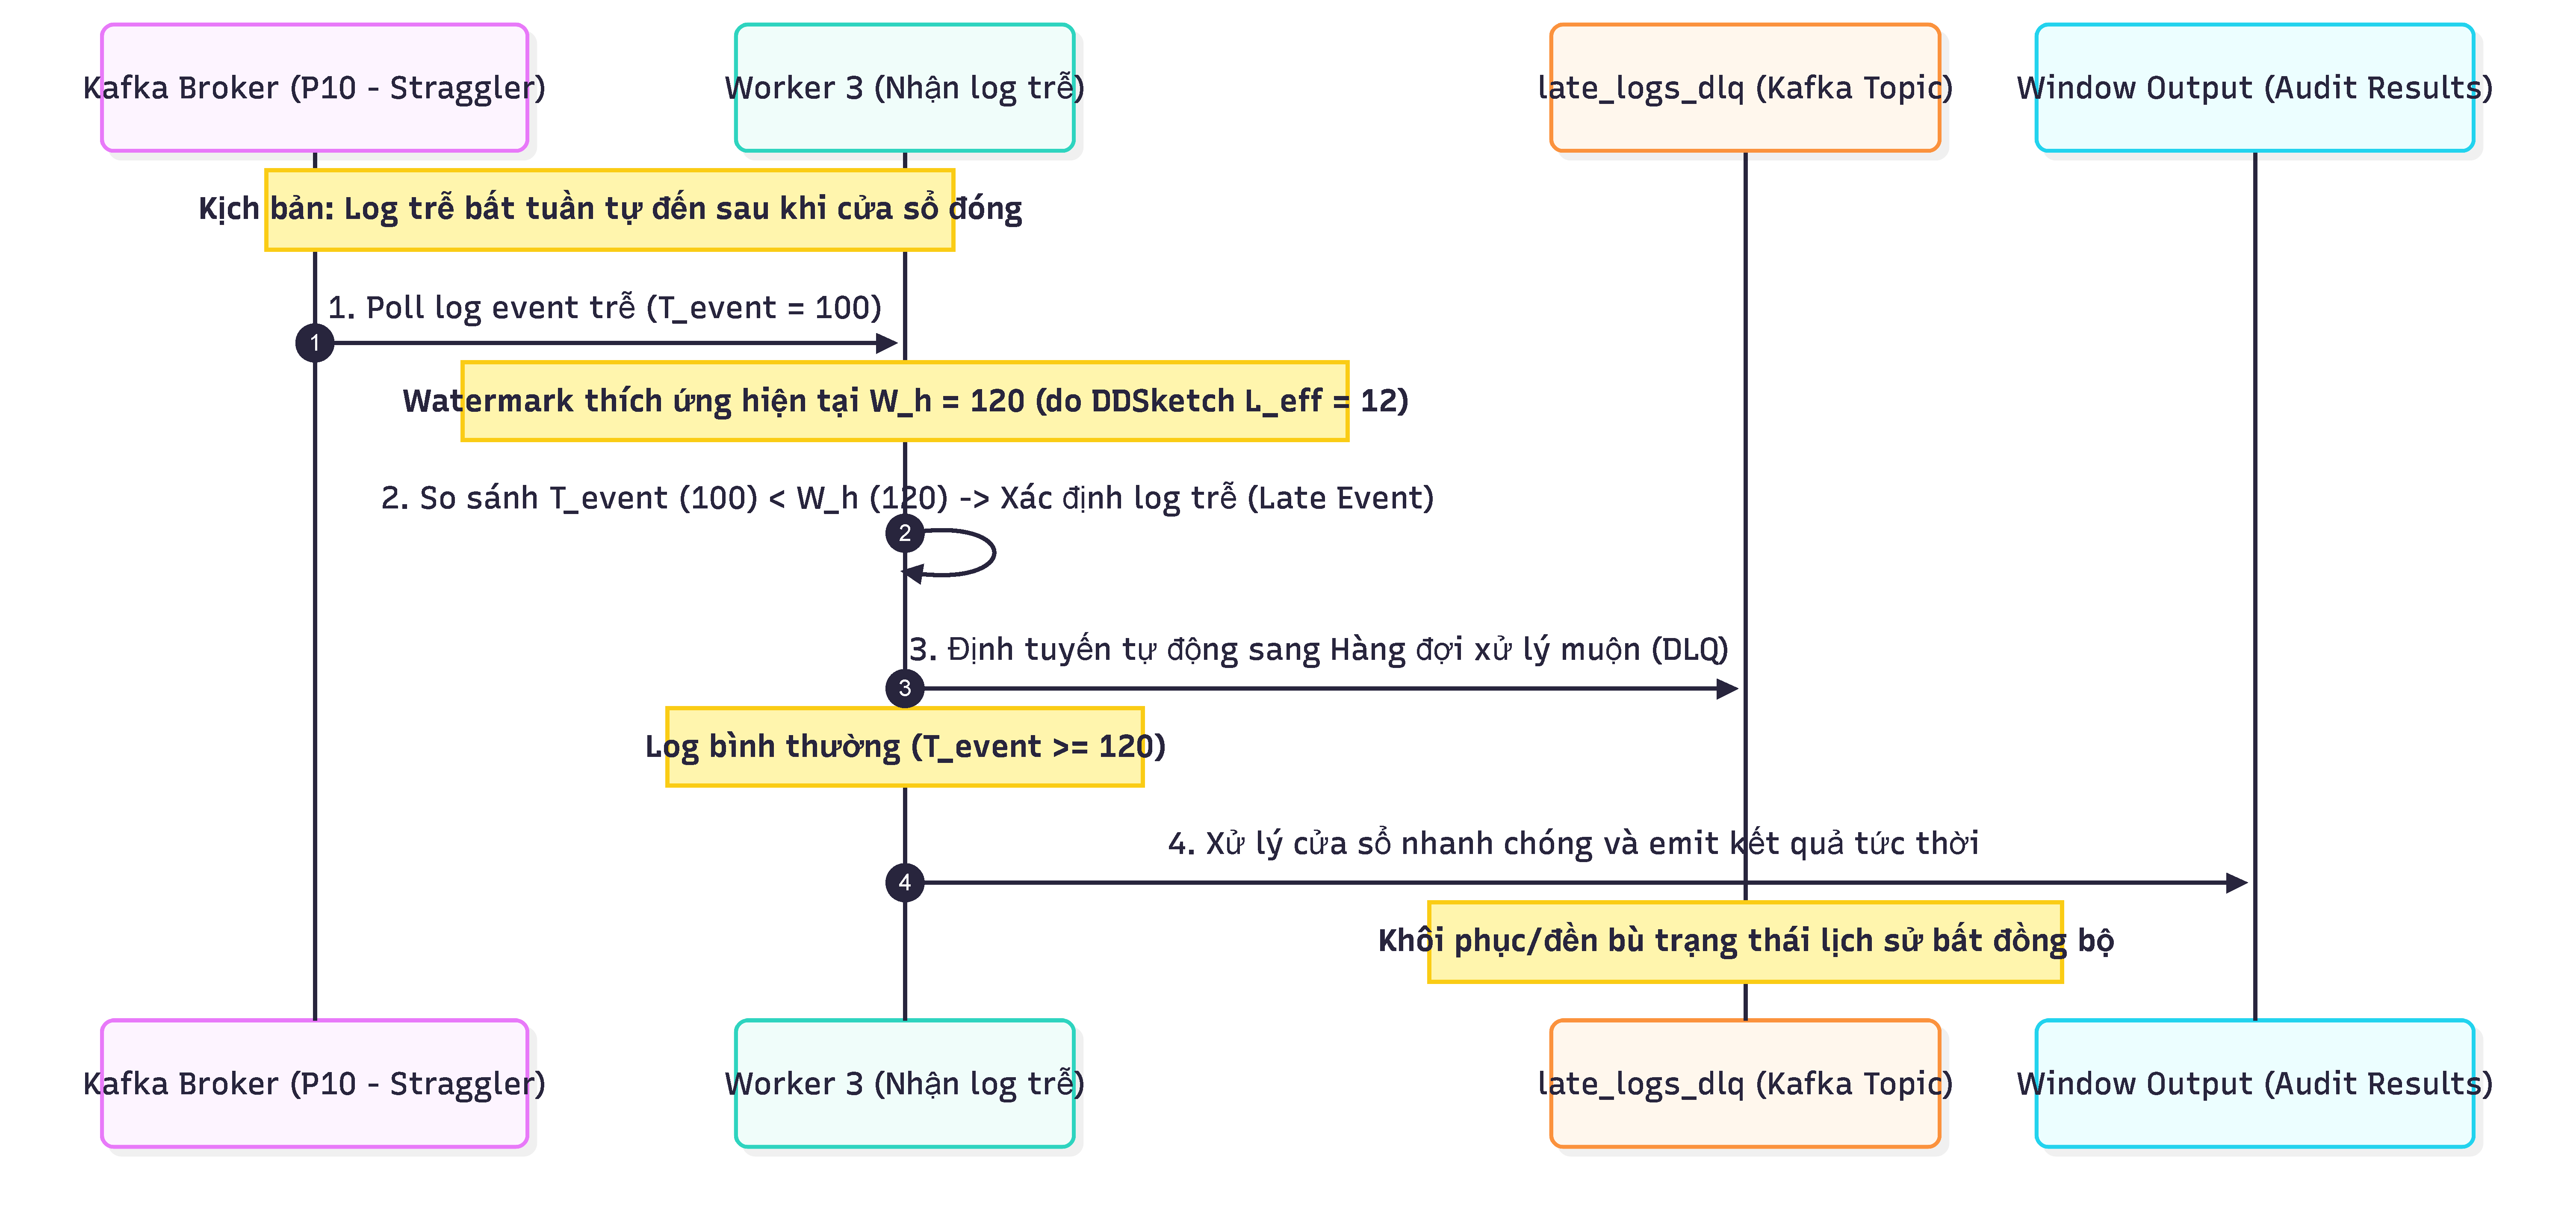
\includegraphics[width=\textwidth,height=11.0cm,keepaspectratio]{DDSketch_DLQ_routing.pdf}
    \caption{Trình tự xử lý Straggler chế độ Heuristic: DDSketch ước lượng \& định tuyến DLQ.}
    \label{fig:ddsketchdlq}
\end{figure}

\vspace{0.5cm}

% ─────────────────────────────────────────────────────────────────────────────
\section{Tech Stack \& Implementation Plan (Công nghệ \& Kế hoạch triển khai)}
% ─────────────────────────────────────────────────────────────────────────────
\begin{itemize}[leftmargin=*]
    \item \textbf{Programming Language (Ngôn ngữ lập trình):} Python 3.10+ (Đảm bảo hiệu năng lập trình nhanh, thư viện phân tích dữ liệu phong phú).
    \item \textbf{Deployment (Phương thức triển khai):}
    Đóng gói bằng \textit{Docker} và điều phối đa container qua \textit{Docker Compose}. Cấu hình hai hồ sơ (profiles) độc lập trong \texttt{docker-compose.yml} để khởi động nhanh chóng hệ thống ở chế độ Strict hoặc Heuristic chỉ với một lệnh duy nhất:
    \begin{itemize}[label={-}]
        \item Strict Profile: Khởi chạy Coordinator và 3 Worker chế độ nghiêm ngặt.
        \item Heuristic Profile: Khởi chạy Aggregator và các Worker chế độ thích ứng trễ.
    \end{itemize}
    \item \textbf{Libraries/Frameworks (Các thư viện cốt lõi):}
    \begin{itemize}[label={-}]
        \item \texttt{grpcio} \& \texttt{grpcio-tools}: Xây dựng giao diện RPC hiệu năng cao.
        \item \texttt{pyrocksdb} hoặc RocksDB binding: Quản lý lưu trữ trạng thái tại Worker.
        \item \texttt{DDSketch} implementation: Thuật toán phân vị thích ứng với sai số giới hạn $\alpha = 0.01$.
        \item \texttt{Pandas}, \texttt{Numpy}, \texttt{Matplotlib}: Thống kê dữ liệu thực nghiệm, tính toán bootstrap CI và vẽ đồ thị Pareto.
        \item \texttt{pytest}: Framework viết kiểm thử tự động (unit test \& integration test).
    \end{itemize}
\end{itemize}

\vspace{0.5cm}

% ─────────────────────────────────────────────────────────────────────────────
\section{Success Metrics \& Analysis (Chỉ số đánh giá \& Phân tích kịch bản sự cố)}
% ─────────────────────────────────────────────────────────────────────────────

\subsection{Completeness-at-Latency Trade-off (Sự đánh đổi giữa tính hoàn thiện dữ liệu và độ trễ)}

Để đánh giá hiệu quả của hai phương thức định thời logic, hệ thống thực hiện đo lường hai chỉ số định lượng cốt lõi:
\begin{enumerate}
    \item \textbf{Tính hoàn thiện dữ liệu (Data Completeness \%)}:
    \begin{itemize}
        \item \textit{Độ hoàn thiện tức thời (Immediate Completeness)}: Tỷ lệ dữ liệu xử lý đúng hạn trong cửa sổ logic trước khi mốc thời gian Watermark đóng cửa sổ đó.
        \item \textit{Độ hoàn thiện cuối cùng (Eventual Completeness)}: Tỷ lệ dữ liệu được tổng hợp đầy đủ sau khi đã tính cả các bản ghi đến muộn được xử lý đền bù qua Hàng đợi xử lý muộn (Dead-Letter Queue - DLQ).
    \end{itemize}
    \item \textbf{Độ trễ chờ Watermark (Watermark Latency / Wait Time)}: Khoảng thời gian hệ thống phải chờ (tính bằng giây mô phỏng) từ lúc cửa sổ thời gian logic kết thúc cho đến khi mốc thời gian Watermark toàn cục vượt qua biên đóng cửa sổ.
\end{enumerate}

Chúng tôi đã thực hiện chạy quét thực nghiệm (benchmark sweeps) trên toàn bộ tập dữ liệu \textbf{2,961,423 dòng} (\texttt{nyc\_taxi\_events\_full.csv}, kích thước khoảng 152 MB). Dưới đây là các phân tích chuyên sâu về sự đánh đổi này.

\subsubsection{Cơ chế nén thời gian mô phỏng (Time Compression Design, DIV = 60)}
Trong dữ liệu thực tế, sự lệch thời gian (skew) giữa thời gian phát sinh sự kiện (event-time) và thời gian hệ thống nhận được dữ liệu (arrival-time) là cực kỳ nhỏ so với tổng thời gian của cả tập dữ liệu (khoảng 31 ngày). Nếu phát lại luồng dữ liệu theo tỷ lệ 1:1, đường cong độ hoàn thiện sẽ luôn phẳng ở mức 100\% do độ trễ đến muộn gần như bằng 0.

Để mô phỏng hành vi bất tuần tự khốc liệt trong môi trường phân tán thực tế, chúng tôi áp dụng hệ số nén thời gian $\text{DIV} = 60$. Công thức ánh xạ mốc thời gian như sau:
{\large
\begin{equation}
    \boxed{\displaystyle T_{\text{event}} = \frac{T_{\text{pickup}} - T_{\text{pickup,min}}}{\text{DIV}}}
\end{equation}
\begin{equation}
    \boxed{\displaystyle T_{\text{arrival}} = \frac{T_{\text{dropoff}} - T_{\text{pickup,min}}}{\text{DIV}}}
\end{equation}
}
Theo đó, độ trễ đến muộn của mỗi sự kiện được bảo toàn nguyên vẹn về mặt tỷ lệ vật lý và chỉ bị co giãn theo hệ số nén:
{\large
\begin{equation}
    \boxed{\displaystyle \text{Lateness} = T_{\text{arrival}} - T_{\text{event}} = \frac{T_{\text{dropoff}} - T_{\text{pickup}}}{\text{DIV}}}
\end{equation}
}
Với cấu hình $\text{DIV} = 60$, các đặc trưng của tập dữ liệu trở nên cực kỳ phù hợp để kiểm thử cơ chế Watermark với kích thước cửa sổ 5 giây:
\begin{itemize}
    \item \textbf{Tỷ lệ bất tuần tự}: Có tới \textbf{49.41\%} tổng số sự kiện (1,463,199 dòng) đến lệch thứ tự so với sự kiện liền kề trước đó.
    \item \textbf{Phân phối độ trễ}: Giá trị trung vị (P50 Lateness) là $11.63$ giây, phân vị P90 là $28.80$ giây, P95 là $37.78$ giây, P99 là $59.70$ giây, và độ trễ ngoại lai lớn nhất lên tới $359.73$ giây.
\end{itemize}

\subsubsection{Kết quả quét thực nghiệm so sánh trực tiếp}
Kết quả so sánh trực tiếp giữa hai chiến lược Strict Watermark và Heuristic Watermark được trình bày trong Bảng~\ref{tab:completeness_latency_tradeoff}.

\begin{table}[H]
    \centering
    \small
    \caption{Kết quả thực nghiệm so sánh sự đánh đổi giữa độ trễ chờ và tính hoàn thiện dữ liệu.}
    \label{tab:completeness_latency_tradeoff}
    \begin{tabular}{r r r r r r}
        \toprule
        \multicolumn{2}{c}{\textbf{Strict Watermark}} & \multicolumn{4}{c}{\textbf{Heuristic Watermark + DLQ}} \\
        \cmidrule(lr){1-2} \cmidrule(lr){3-6}
        \textbf{$\delta$ = Wait (s)}
          & \textbf{Completeness (\%)}
          & \textbf{Phân vị $p$}
          & \textbf{$L_{\text{eff}}$ (s)}
          & \textbf{Tức thời (\%)}
          & \textbf{Cuối cùng (\%)} \\
        \midrule
        \rowcolor{white}
        \textbf{0}
          & \textbf{8.75}
          & 0.500 & 11.63 & 64.21 & 100.00 \\
        1   & 12.88 & 0.500 & 11.63 & 64.21 & 100.00 \\
        2   & 17.86 & 0.500 & 11.63 & 64.21 & 100.00 \\
        3   & 23.29 & 0.500 & 11.63 & 64.21 & 100.00 \\
        5   & 34.66 & 0.500 & 11.63 & 64.21 & 100.00 \\
        7   & 45.48 & 0.500 & 11.63 & 64.21 & 100.00 \\
        10  & 59.17 & 0.500 & 11.63 & 64.21 & 100.00 \\
        15  & 75.03 & 0.500 & 11.63 & 64.21 & 100.00 \\
        \cmidrule{3-6}
        20  & 84.44 & 0.750 & 18.67 & 81.26 & 100.00 \\
        30  & 93.23 & 0.900 & 28.80 & 91.31 & 100.00 \\
        40  & 96.72 & 0.950 & 37.78 & 94.77 & 100.00 \\
        50  & 98.41 & 0.990 & 59.70 & 97.70 & 100.00 \\
        60  & 99.27 & 0.990 & 59.70 & 97.70 & 100.00 \\
        90  & 99.89 & 0.999 & 95.03 & 98.38 & 100.00 \\
        120 & 99.97 & 0.999 & 95.03 & 98.38 & 100.00 \\
        \bottomrule
    \end{tabular}
    \\[4pt]
    {\footnotesize Ghi chú: Cột \textbf{Cuối cùng (\%)} luôn đạt 100\% nhờ cơ chế đối chiếu đền bù qua Hàng đợi xử lý muộn (DLQ).}
\end{table}

\textbf{Giải thích các cột trong Bảng~\ref{tab:completeness_latency_tradeoff}:}
\begin{itemize}[leftmargin=*]
    \item \textbf{Wait (s)}: Thời gian chờ (Wait Time) hay biên an toàn $\delta$ (DELTA\_BASE\_S) mà hệ thống Strict Watermark áp đặt sau khi cửa sổ logic kết thúc trước khi chốt kết quả. Đây chính là khoảng trễ nhân tạo để chờ các sự kiện đến muộn.
    \item \textbf{Strict \%}: Độ hoàn thiện dữ liệu tức thời (Immediate Completeness) của chế độ Strict Watermark, tương ứng với mức Wait Time ở cột đầu tiên. Thể hiện tỷ lệ phần trăm dữ liệu được xử lý đúng hạn trong cửa sổ trước khi Watermark đóng.
    \item \textbf{$p$}: Phân vị mục tiêu (Target Quantile) sử dụng trong chế độ Heuristic Watermark. $p = 0.50$ nghĩa là ước lượng trung vị của phân phối độ trễ; $p = 0.999$ nghĩa là gần như toàn bộ phân phối (99.9\%).
    \item \textbf{$L_{\text{eff}}$ (s)}: Độ trễ hiệu dụng (Effective Latency) được ước lượng trực tuyến bởi cấu trúc DDSketch tại phân vị $p$ tương ứng. Đây là ngưỡng thời gian mà Heuristic Watermark dùng để chốt cửa sổ thay vì dùng giá trị cố định $\delta$ như chế độ Strict.
    \item \textbf{Imm.\,\%}: Độ hoàn thiện dữ liệu tức thời (Immediate Completeness) của chế độ Heuristic Watermark tại phân vị $p$ và $L_{\text{eff}}$ tương ứng. Dữ liệu đến sau khi cửa sổ đã chốt sẽ bị định tuyến sang DLQ.
    \item \textbf{Eventual\,\%}: Độ hoàn thiện dữ liệu cuối cùng (Eventual Completeness) của chế độ Heuristic Watermark sau khi đã đối chiếu đền bù toàn bộ dữ liệu từ Hàng đợi xử lý muộn (DLQ). Giá trị luôn đạt \textbf{100\%} chứng minh rằng cơ chế DLQ đảm bảo không mất mát dữ liệu.
\end{itemize}

\subsubsection{Các phát hiện và Phân tích chuyên sâu từ thực nghiệm}
\begin{enumerate}
    \item \textbf{Mô hình hóa đường cong và Chi phí biên (Marginal Cost Analysis)}:
    Đường cong độ hoàn thiện thực nghiệm của Strict Watermark bám rất sát hàm phân phối tích lũy CDF của độ trễ thực tế ($R^2 \approx 0.876$). Phân tích chi phí biên (Wait Time cần thiết để tăng $1\%$ độ hoàn thiện) chỉ ra quy luật lợi ích giảm dần cực kỳ rõ rệt:
    \begin{itemize}
        \item Trong khoảng $\delta$ từ $0$ đến $10$ giây, chi phí biên rất thấp, chỉ mất khoảng \textbf{176 đến 242 ms} thời gian chờ cho mỗi $1\%$ dữ liệu thu hồi thêm.
        \item Khi tiệm cận mức hoàn thiện cao, chi phí biên tăng vọt một cách phi tuyến tính. Để tăng độ hoàn thiện từ $99.0\%$ lên $99.9\%$ (chênh lệch chỉ $0.9\%$), hệ thống phải tăng $\delta$ từ $60$s lên $120$s, tức chi phí biên lên tới \textbf{66,666 ms chờ đợi cho mỗi 1\% hoàn thiện}.
        \item Để đạt độ hoàn thiện tuyệt đối (tránh mất mát 833 sự kiện ngoại lai có độ trễ $>120$s), thời gian trễ bắt buộc phải cấu hình $\delta \ge 360$ giây. Đây là mức trễ không thể chấp nhận được đối với các hệ thống phân tích thời gian thực.
    \end{itemize}

    \item \textbf{Cơ chế thích ứng động của Heuristic Watermark qua DDSketch}:
    Chế độ Heuristic giải phóng hệ thống khỏi sự phụ thuộc vào cấu hình tĩnh bằng cách sử dụng cấu trúc dữ liệu phác thảo DDSketch ($\alpha = 0.01$) để tính toán động độ trễ hiệu dụng $L_{\text{eff}}$ (streaming quantiles) từ dòng dữ liệu thực tế:
    \begin{itemize}
        \item Quá trình hội tụ trực tuyến của $L_{\text{eff}}$ diễn ra rất mượt mà và ổn định. Với phân vị đích $p = 0.90$, giá trị $L_{\text{eff}}$ bắt đầu ở $27.77$s sau 50,000 sự kiện đầu tiên và hội tụ chính xác về $28.80$s ở cuối luồng dữ liệu.
        \item Tại $p = 0.50$, hệ thống tự động duy trì thời gian chờ $L_{\text{eff}} \approx 11.63$ giây (nhỏ hơn 10 lần so với mức $\delta = 120$s của Strict để đạt cùng mức hoàn thiện cuối cùng).
        \item Dù độ hoàn thiện tức thời chỉ đạt khoảng $64.21\%$, cơ chế đối chiếu đền bù qua Hàng đợi xử lý muộn (DLQ) đảm bảo \textbf{tính hoàn thiện cuối cùng đạt tuyệt đối 100\%} mà không gây tắc nghẽn hay trì hoãn các cửa sổ xử lý chính.
    \end{itemize}

    \item \textbf{Ảnh hưởng của kích thước cửa sổ (Window Size Sensitivity Analysis)}:
    Thực nghiệm quét nhạy cảm cho thấy kích thước cửa sổ lớn hơn (ví dụ từ 1s tăng lên 60s) làm giảm số lượng cửa sổ logic và giảm thiểu sai số biên ở các điểm đóng cửa sổ, từ đó tăng độ hoàn thiện tự nhiên khi không chờ ($\delta = 0$s tăng từ $2.34\%$ lên $77.76\%$). Tuy nhiên, đối với các trường hợp $\delta \ge 40$s, đường cong độ hoàn thiện hội tụ về cùng một dạng phân phối bất kể kích thước cửa sổ, chứng tỏ phân phối độ trễ dòng sự kiện mới là yếu tố quyết định hiệu năng.
\end{enumerate}

\subsubsection{Khuyến nghị cấu hình vận hành thực tế (Production Guidelines)}
Dựa trên kết quả thực nghiệm, chúng tôi đề xuất các mô hình cấu hình tối ưu tùy thuộc vào mục tiêu nghiệp vụ của hệ thống:
\begin{itemize}
    \item \textbf{Dashboard trực quan thời gian thực (Real-time Dashboards)}: Sử dụng chế độ Strict Watermark với $\delta = 38$s. Mô hình này cung cấp độ hoàn thiện tức thời $\approx 95\%$ với độ trễ xử lý cố định và dễ dự đoán, loại bỏ hoàn toàn chi phí xử lý đền bù phức tạp của DLQ.
    \item \textbf{Hệ thống phân tích và đối chiếu tài chính (Analytics/Financial Ledgers)}: Sử dụng chế độ Heuristic Watermark với phân vị $p = 0.50$ ($L_{\text{eff}} \approx 12$s). Cấu hình này giúp đóng cửa sổ nhanh nhất, giải phóng trạng thái trong RocksDB ngay lập tức, trong khi DLQ đảm bảo tính chính xác và đầy đủ tuyệt đối $100\%$ của dữ liệu.
    \item \textbf{Chế độ vận hành cân bằng (Balanced Operations)}: Sử dụng chế độ Heuristic Watermark với phân vị $p = 0.90$ ($L_{\text{eff}} \approx 29$s). Lựa chọn này đem lại độ hoàn thiện tức thời cao ($91.31\%$), do đó lượng dữ liệu trễ phải đi qua DLQ chỉ chiếm dưới $10\%$, giảm thiểu tối đa tài nguyên tính toán cho pha đền bù dữ liệu.
\end{itemize}

\subsection{Failure Scenarios \& Recovery Path (Kịch bản sự cố \& Quy trình phục hồi)}
\begin{enumerate}
        \item \textit{Sập Worker Node (Worker Node Crash)}:
        \begin{itemize}[label={-}]
            \item \textbf{Sự cố (Failure Scenario)}: Khi một Worker (ví dụ: Worker 3 phụ trách các phân mảnh $P_9 - P_{11}$) bị dừng tiến trình đột ngột:
            \begin{itemize}
                \item \textbf{Phát hiện lỗi}: Coordinator không nhận được nhịp tim \texttt{WorkerPing} từ Worker 3 quá 10 giây (\texttt{HEARTBEAT\_TIMEOUT\_S}), lập tức xác nhận Worker 3 đã sập.
                \item \textbf{Phong tỏa và Đổi Term (Fencing)}: Coordinator tăng giá trị \texttt{fencing term} logic lên để vô hiệu hóa tất cả các lệnh cũ từ Worker 3 nếu nó sống dậy bất ngờ.
                \item \textbf{Tái phân bổ \& Cân bằng tải (Rebalance)}: Coordinator đổi trạng thái các phân mảnh $P_9, P_{10}, P_{11}$ sang \texttt{REASSIGNING} trong Raft log. Để đảm bảo cân bằng tải và tránh hiện tượng nút cổ chai, Coordinator không chỉ định một node duy nhất gánh toàn bộ, mà thực hiện chia đều các phân mảnh bị ảnh hưởng cho các Worker còn sống:
                \begin{itemize}[label={-}]
                    \item Phân mảnh $P_9$ được gánh hộ bởi Worker 0 (node0).
                    \item Phân mảnh $P_{10}$ được gánh hộ bởi Worker 1 (node1).
                    \item Phân mảnh $P_{11}$ được gánh hộ bởi Worker 2 (node2).
                \end{itemize}
                \item \textbf{Khôi phục trạng thái ấm (Warm State Recovery)}: Các Worker còn sống (Worker 0, Worker 1, Worker 2) khi nhận chỉ thị tiếp quản phân mảnh tương ứng sẽ nạp checkpoint từ Shared Volume (Tier-2) bao gồm offset đã xử lý gần nhất và metadata RocksDB, thực hiện \texttt{seek(checkpoint\_offset + 1)} trên Kafka để tiếp tục xử lý dòng sự kiện, bảo đảm tính nhất quán Exactly-Once.
            \end{itemize}
            \item \textbf{Phục hồi (Recovery Path - Failback)}: Khi Worker 3 được khởi động lại và sẵn sàng nhận lại các phân mảnh cũ của mình ($P_9, P_{10}, P_{11}$):
            \begin{itemize}
                \item \textbf{Bước 1 (Request)}: Worker 3 gửi yêu cầu đăng ký reassign các phân mảnh cũ lên Coordinator.
                \item \textbf{Bước 2 (Lock)}: Coordinator ghi nhận trạng thái \texttt{REASSIGNING} cho các phân mảnh $P_9, P_{10}, P_{11}$ vào Raft log.
                \item \textbf{Bước 3 (Pause Source)}: Coordinator gửi lệnh \texttt{PAUSE} đồng thời đến các Worker đang gánh hộ tạm thời (Worker 0, Worker 1, và Worker 2). Các Worker này dừng kéo dữ liệu từ Kafka cho phân mảnh bàn giao tương ứng, thực hiện flush toàn bộ window state của RocksDB xuống đĩa, ghi checkpoint hoàn chỉnh lên Shared Volume và gửi ack xác nhận kèm offset cuối cùng đã xử lý về Coordinator.
                \item \textbf{Bước 4 (Reassign)}: Coordinator cập nhật trạng thái Kafka consumer group để Worker 3 làm owner mới cho các phân mảnh $P_9 - P_{11}$, thu hồi quyền xử lý từ các Worker đang gánh hộ, ghi nhận trạng thái \texttt{PAUSED} vào Raft log.
                \item \textbf{Bước 5 (Resume Target)}: Coordinator gửi lệnh \texttt{RESUME} kèm \texttt{fencing term} cho Worker 3. Worker 3 nạp checkpoint từ Shared Volume, \texttt{seek(offset + 1)} trên Kafka cho cả 3 phân mảnh, và bắt đầu tiêu thụ dữ liệu bình thường. Trạng thái các phân mảnh đổi về \texttt{ASSIGNED} trong Raft log.
            \end{itemize}
        \end{itemize}
        
        Sơ đồ máy trạng thái phân mảnh (Partition State Machine):
        \begin{figure}[H]
            \centering
            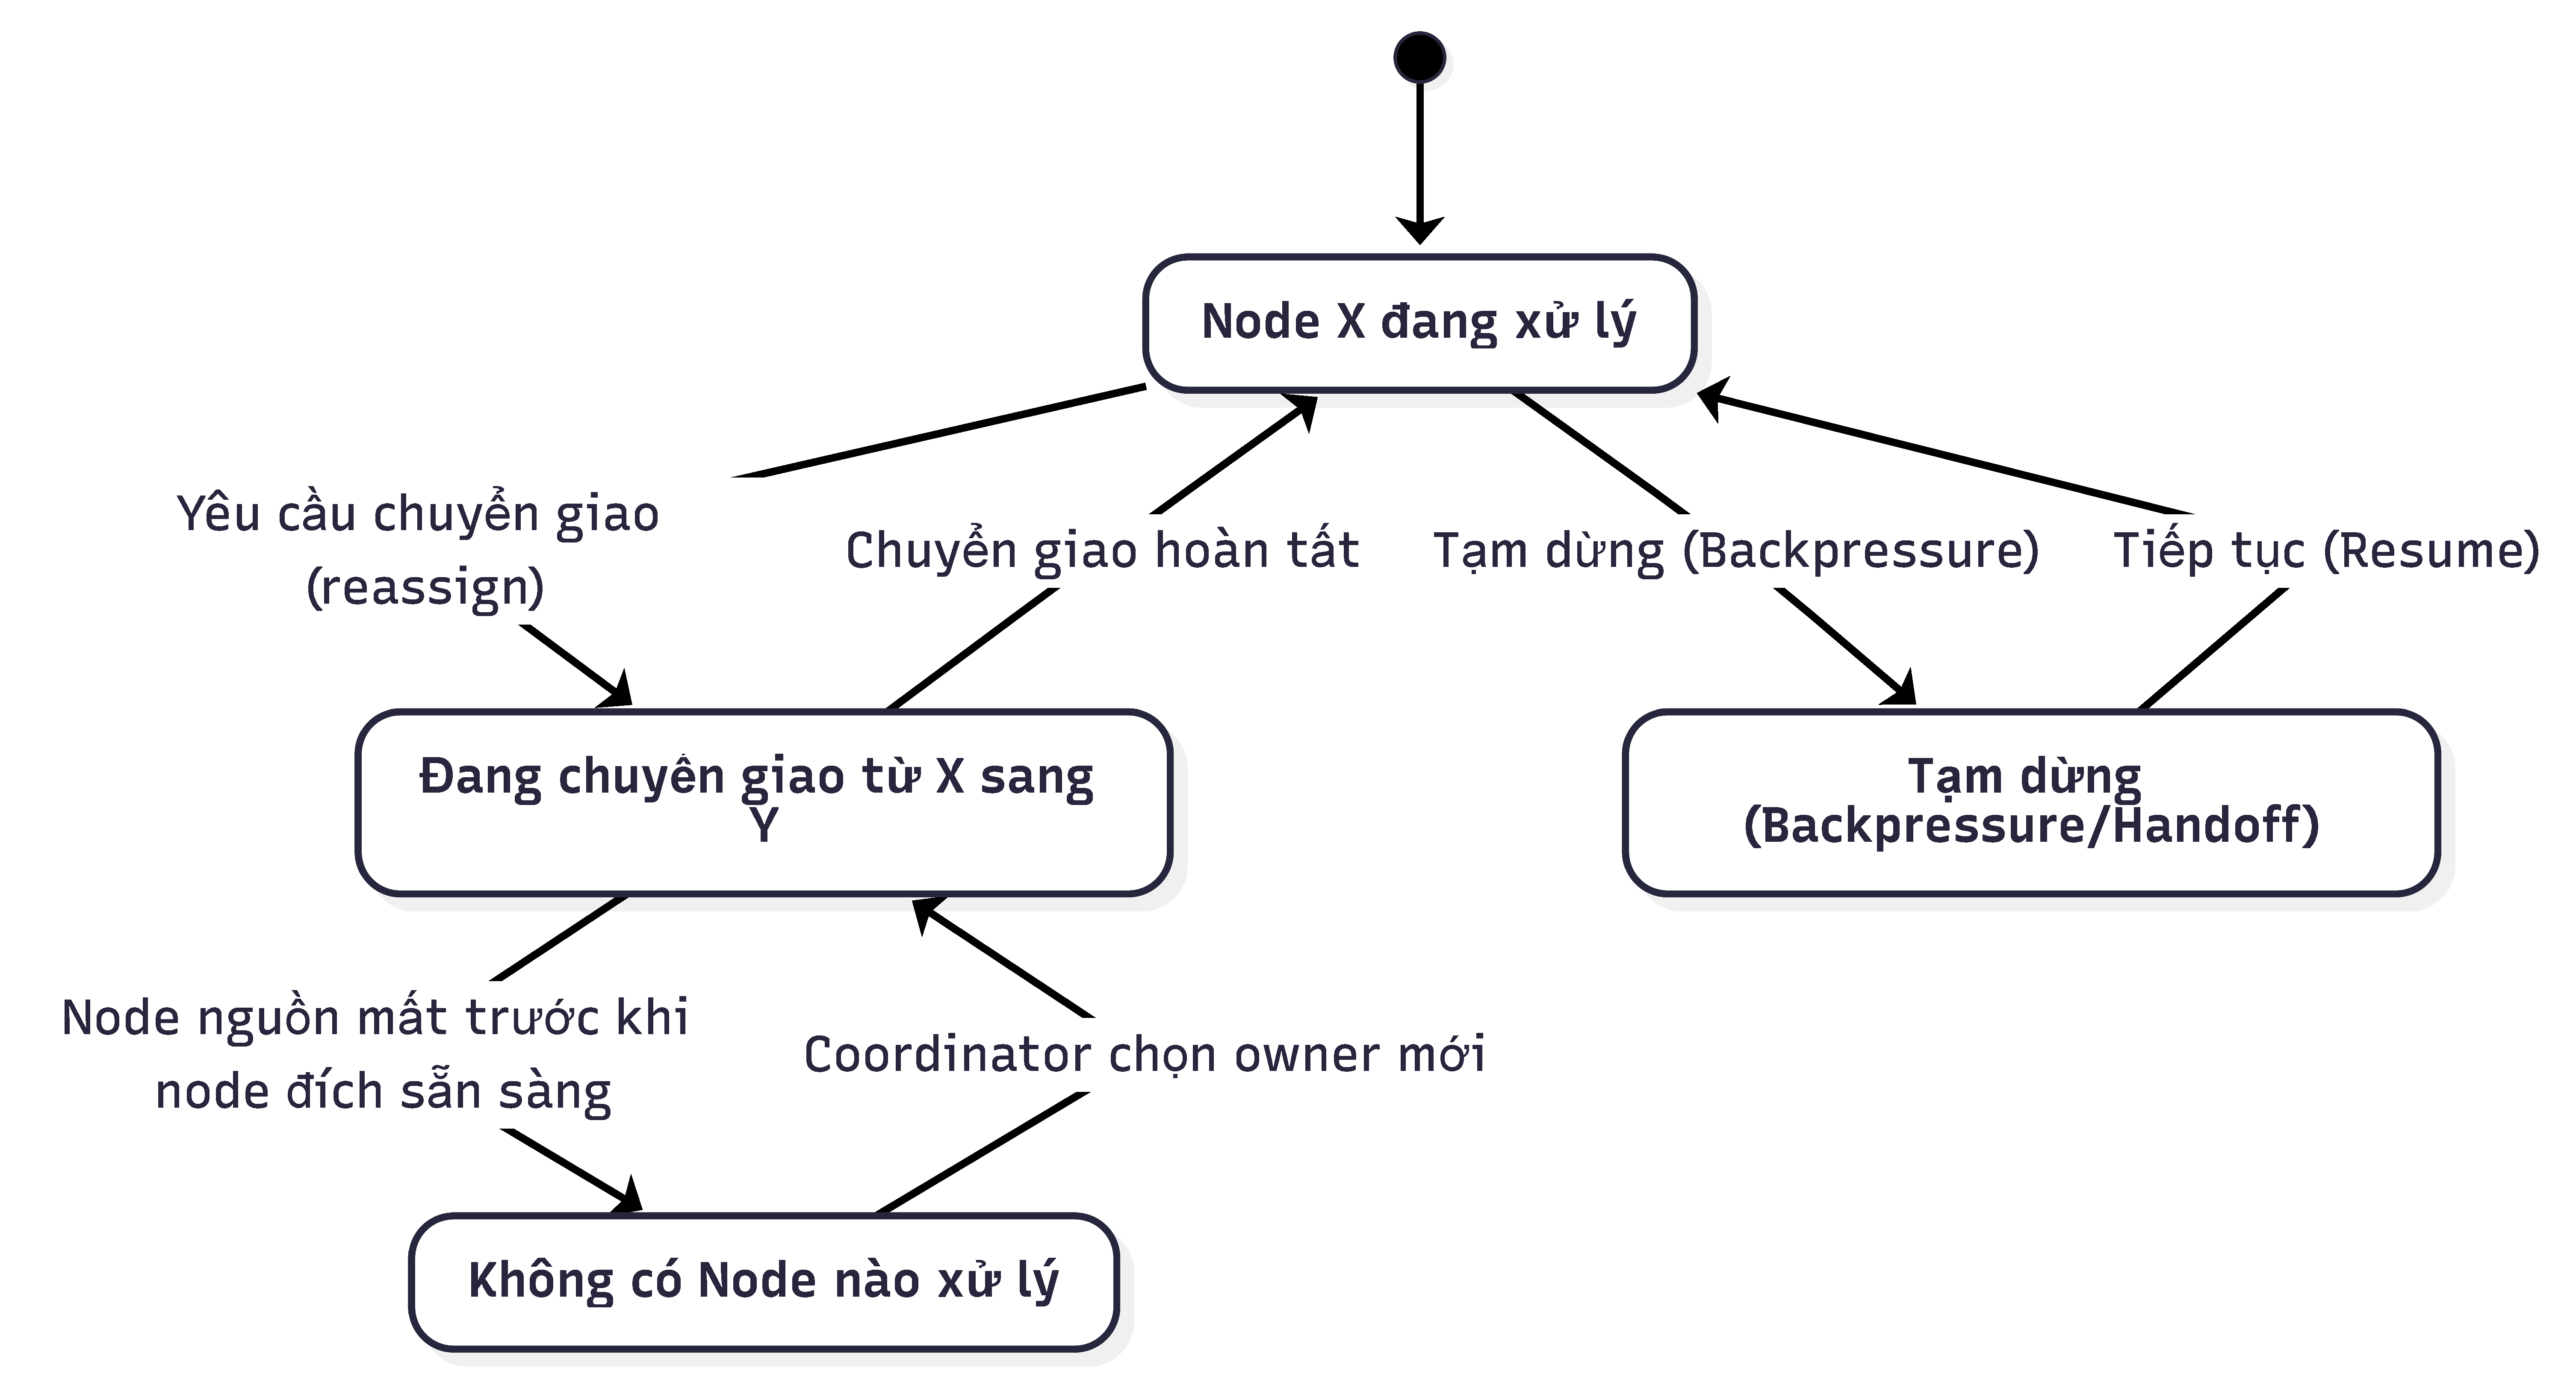
\includegraphics[width=\textwidth,height=9.0cm,keepaspectratio]{Partition State Machine.pdf}
            \caption{Sơ đồ máy trạng thái phân mảnh (Partition State Machine).}
            \label{fig:partitionstatemachine}
        \end{figure}

        Sơ đồ trình tự Failback 5 bước sau phục hồi:
        \begin{figure}[H]
            \centering
            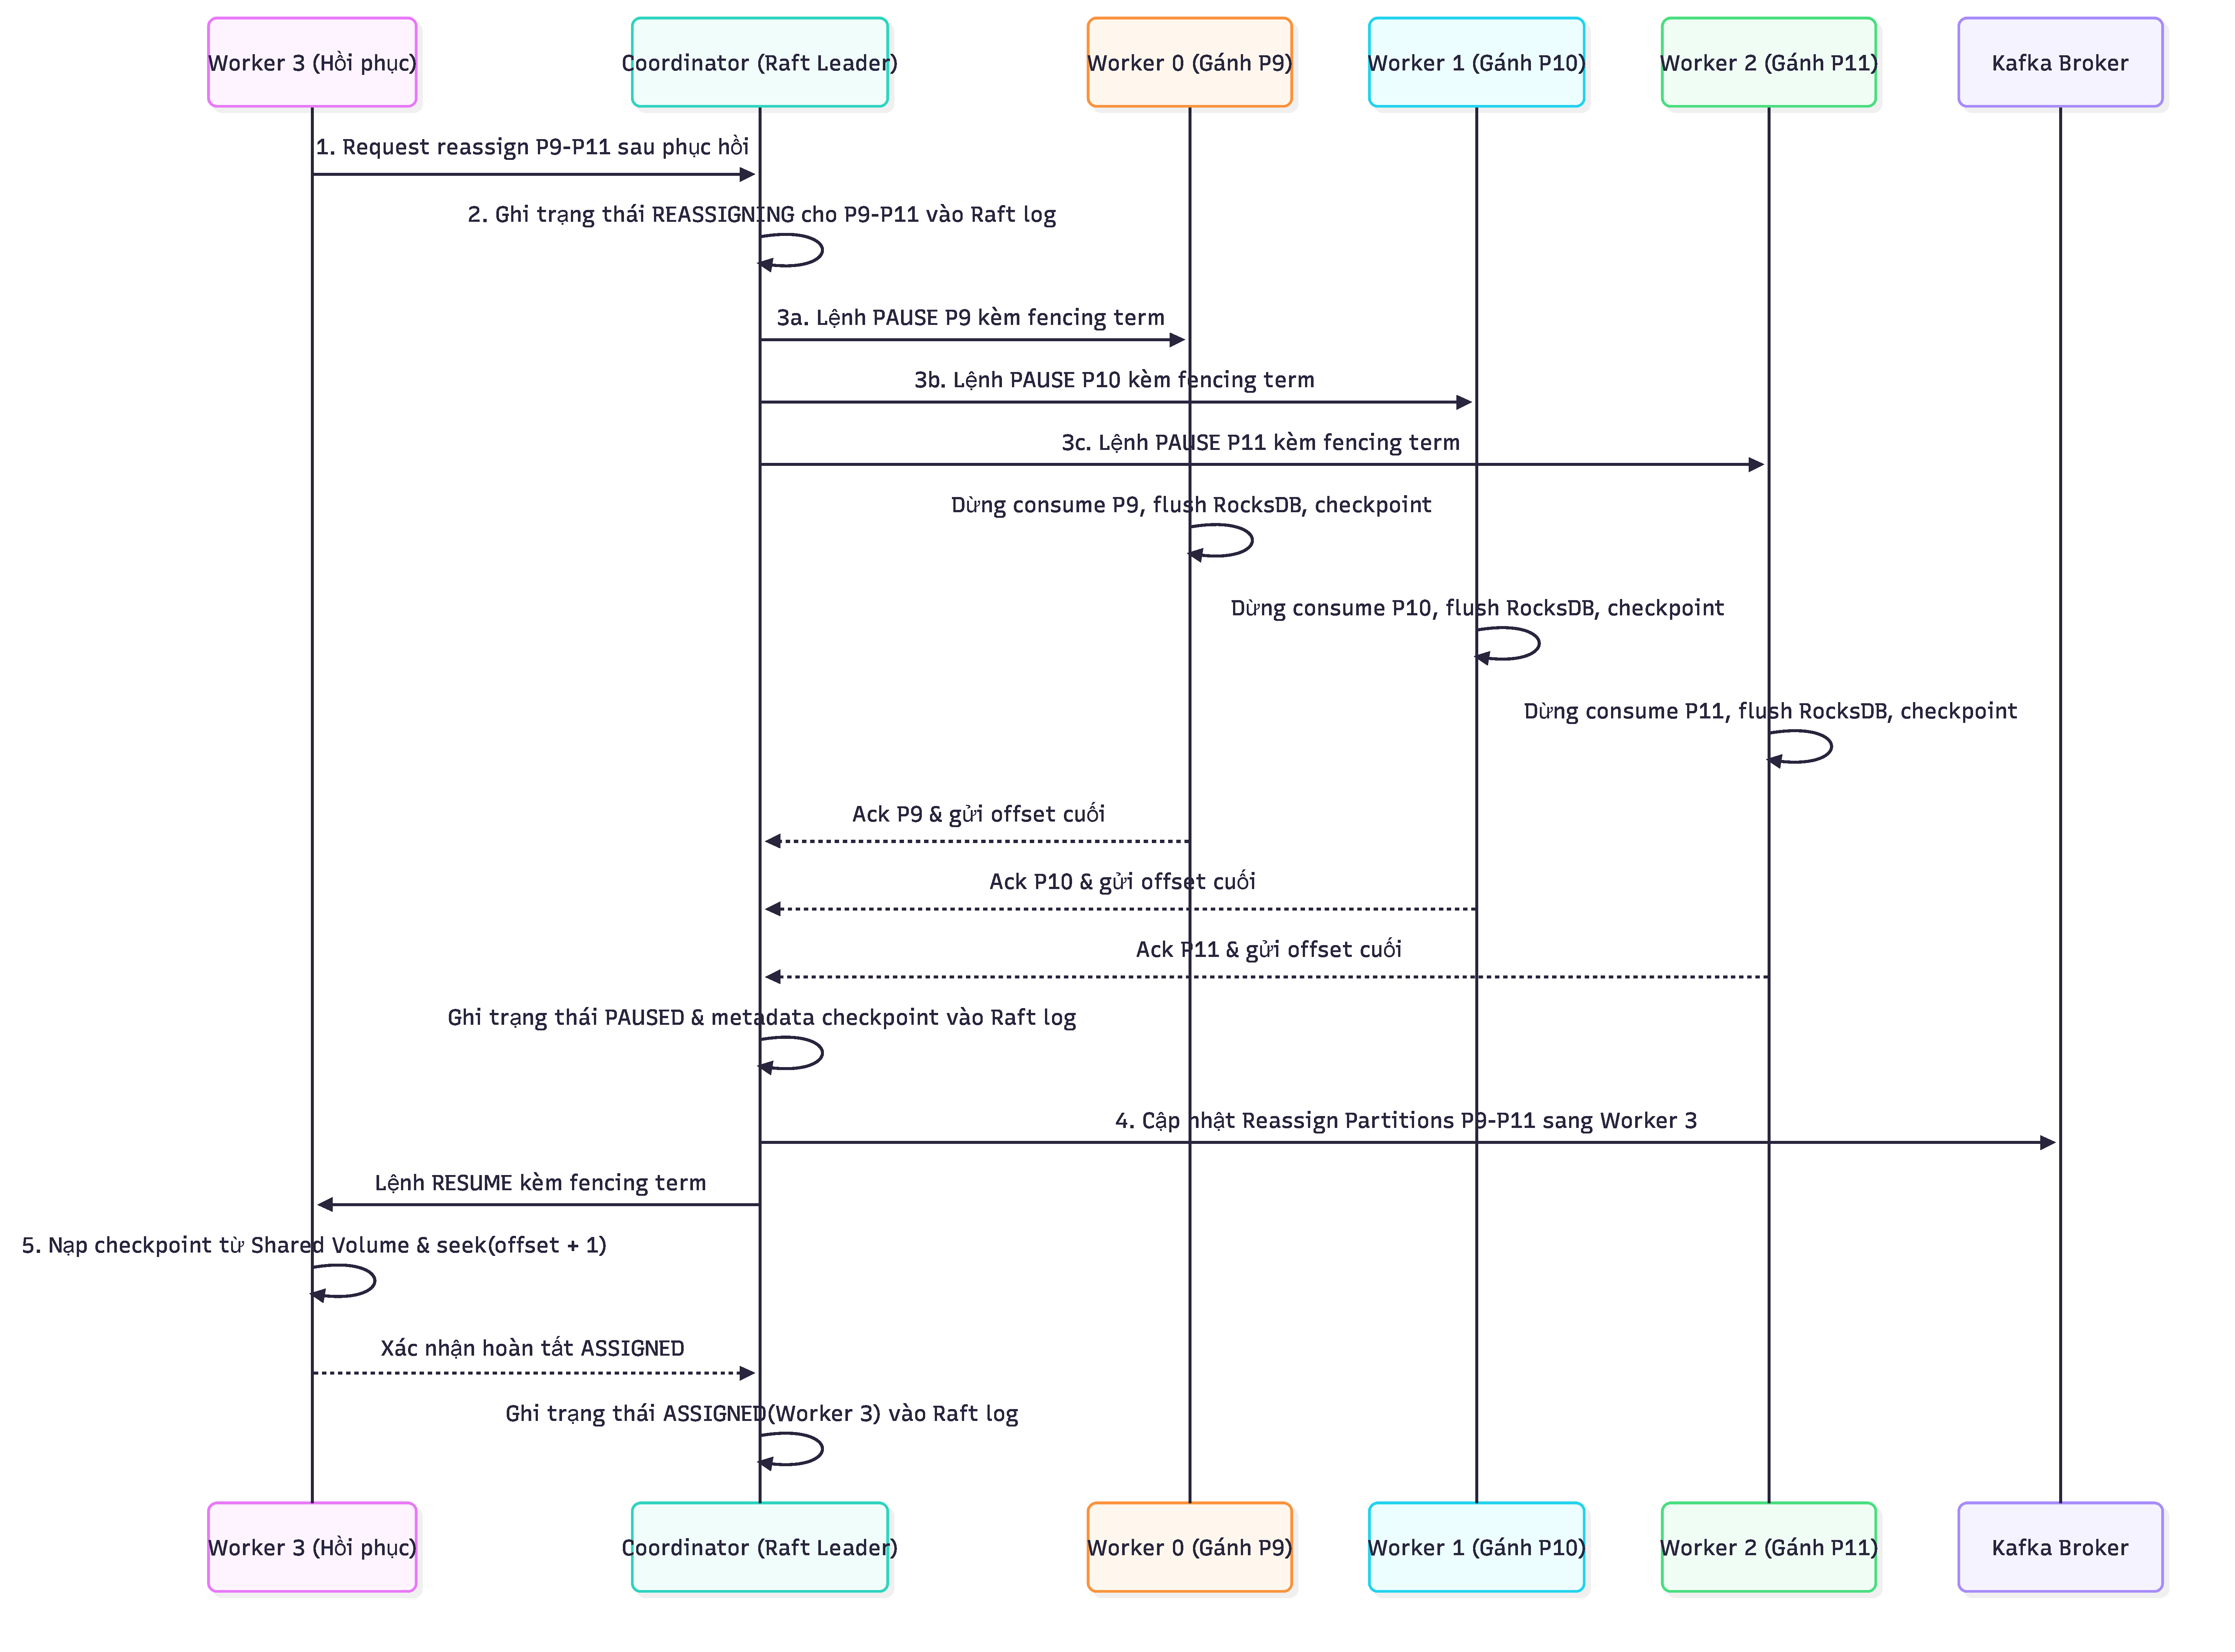
\includegraphics[width=\textwidth,height=11.0cm,keepaspectratio]{5-Step Failback Sequence Diagram.pdf}
            \caption{Sơ đồ trình tự Failback 5 bước sau phục hồi.}
            \label{fig:failbacksequence}
        \end{figure}

        \item \textit{Phân mảnh mạng (Split-brain Fencing)}: Sử dụng cặp Fencing Token gồm nhiệm kỳ độc bản (\texttt{fencing term}) trên các chỉ thị điều phối để ngăn chặn các Coordinator cũ gửi lệnh sai lệch tới Worker khi mạng bị chia cắt.
        \item \textit{Hiện tượng Idle Partition}: Giả lập phân mảnh 10 không có log phát sinh. Worker phải tự động đánh dấu phân mảnh này là \texttt{TEMPORARY\_IDLE} dựa trên cấu hình timeout để Coordinator tạm thời loại trừ khỏi hàm $\min$ tính $W_{global}$, ngăn chặn hiện tượng nghẽn dòng chảy thời gian của cả hệ thống.
    \end{enumerate}
\end{itemize}

\vspace{0.5cm}

% ─────────────────────────────────────────────────────────────────────────────
\section{Project Milestones (Mốc thời gian Dự án)}
% ─────────────────────────────────────────────────────────────────────────────
Kế hoạch triển khai dự án chi tiết kéo dài trong 12 tuần học:
\begin{itemize}[leftmargin=*]
    \item \textbf{Milestone 1 (Tuần 5): Khởi tạo môi trường \& Ingestion Pipeline}
    \begin{itemize}[label={-}]
        \item Hoàn thành cấu hình Dockerfile và môi trường gRPC/REST.
        \item Hiện thực hóa module Ingestor và chiến lược phân mảnh dữ liệu ngang bằng hàm băm.
        \item Cài đặt Min-Heap ưu tiên sắp xếp sự kiện bất tuần tự tại Worker Node.
    \end{itemize}
    \item \textbf{Milestone 2 (Tuần 8): Hiện thực hóa chế độ Strict Watermark \& Checkpoint}
    \begin{itemize}[label={-}]
        \item Hoàn thành cơ chế phát Punctuation Token thời gian thực và Empty Punctuation khi nhàn rỗi.
        \item Tích hợp RocksDB cục bộ tại các Worker phục vụ lưu trữ trạng thái cửa sổ.
        \item Xây dựng Coordinator Leader điều phối toàn cục và lưu trữ siêu dữ liệu bằng máy trạng thái Raft.
    \end{itemize}
    \item \textbf{Milestone 3 (Tuần 12): Hiện thực hóa Heuristic thích ứng \& Đánh giá thực nghiệm}
    \begin{itemize}[label={-}]
        \item Tích hợp bộ ước lượng DDSketch trực tuyến và cơ chế tự động nâng phân vị khi quá tải mạng.
        \item Hiện thực hóa đường ống sửa lỗi dữ liệu muộn (DLQ Correction path) cập nhật dữ liệu lịch sử.
        \item Viết suite kiểm thử tự động các kịch bản sự cố (Node failure, split-brain, idle partition).
        \item Thực hiện chạy thực nghiệm trên tập dữ liệu 2.96 triệu bản ghi và xuất báo cáo Pareto học thuật hoàn chỉnh.
    \end{itemize}
\end{itemize}

\end{document}
